
% Licensed to the Apache Software Foundation (ASF) under one or more
% contributor license agreements.  See the NOTICE file distributed with
% this work for additional information regarding copyright ownership.
% The ASF licenses this file to You under the Apache License, Version 2.0
% (the "License"); you may not use this file except in compliance with
% the License.  You may obtain a copy of the License at
%
%     http://www.apache.org/licenses/LICENSE-2.0
%
% Unless required by applicable law or agreed to in writing, software
% distributed under the License is distributed on an "AS IS" BASIS,
% WITHOUT WARRANTIES OR CONDITIONS OF ANY KIND, either express or implied.
% See the License for the specific language governing permissions and
% limitations under the License.

\documentclass[11pt]{report}
\title{Apache Accumulo User Manual\\
Version 1.4}
\usepackage{alltt}
\usepackage{multirow}
\usepackage{graphicx}
\usepackage[T1]{fontenc}
\renewcommand{\ttdefault}{txtt}
%\def\verbatim{%
%	\def\verbatim@font{\small\ttfamily}%
%	\verbatim}

\setlength{\textwidth}{6.25in}
\evensidemargin=0in
\oddsidemargin=0in

\usepackage{parskip}
\usepackage{hyperref}
\newenvironment{shellcommands}[0]
{\ttfamily \begin{flushleft} \setlength{\parindent}{0cm} \setlength{\parskip}{12mm} \hangindent=1cm}
{\end{flushleft} \setlength{\parindent}{7mm} \hangindent=0cm \normalfont}

\begin{document}
\maketitle
\tableofcontents

% Licensed to the Apache Software Foundation (ASF) under one or more
% contributor license agreements.  See the NOTICE file distributed with
% this work for additional information regarding copyright ownership.
% The ASF licenses this file to You under the Apache License, Version 2.0
% (the "License"); you may not use this file except in compliance with
% the License.  You may obtain a copy of the License at
%
%     http://www.apache.org/licenses/LICENSE-2.0
%
% Unless required by applicable law or agreed to in writing, software
% distributed under the License is distributed on an "AS IS" BASIS,
% WITHOUT WARRANTIES OR CONDITIONS OF ANY KIND, either express or implied.
% See the License for the specific language governing permissions and
% limitations under the License.

\chapter{Introduction}
Apache Accumulo is a highly scalable structured store based on Google's BigTable.
Accumulo is written in Java and operates over the Hadoop Distributed File System
(HDFS), which is part of the popular Apache Hadoop project. Accumulo supports
efficient storage and retrieval of structured data, including queries for ranges, and
provides support for using Accumulo tables as input and output for MapReduce
jobs.

Accumulo features automatic load-balancing and partitioning, data compression
and fine-grained security labels.



% Licensed to the Apache Software Foundation (ASF) under one or more
% contributor license agreements.  See the NOTICE file distributed with
% this work for additional information regarding copyright ownership.
% The ASF licenses this file to You under the Apache License, Version 2.0
% (the "License"); you may not use this file except in compliance with
% the License.  You may obtain a copy of the License at
%
%     http://www.apache.org/licenses/LICENSE-2.0
%
% Unless required by applicable law or agreed to in writing, software
% distributed under the License is distributed on an "AS IS" BASIS,
% WITHOUT WARRANTIES OR CONDITIONS OF ANY KIND, either express or implied.
% See the License for the specific language governing permissions and
% limitations under the License.

\chapter{Accumulo Design}

\section{Data Model}

Accumulo provides a richer data model than simple key-value stores, but is not a
fully relational database. Data is represented as key-value pairs, where the key and
value are comprised of the following elements:

\begin{center}
$\begin{array}{|c|c|c|c|c|c|} \hline
\multicolumn{5}{|c|}{\mbox{Key}} & \multirow{3}{*}{\mbox{Value}}\\ \cline{1-5}
\multirow{2}{*}{\mbox{Row ID}}& \multicolumn{3}{|c|}{\mbox{Column}} & \multirow{2}{*}{\mbox{Timestamp}} & \\ \cline{2-4}
& \mbox{Family} & \mbox{Qualifier} & \mbox{Visibility} & & \\ \hline
\end{array}$
\end{center}

All elements of the Key and the Value are represented as byte arrays except for
Timestamp, which is a Long. Accumulo sorts keys by element and lexicographically
in ascending order. Timestamps are sorted in descending order so that later
versions of the same Key appear first in a sequential scan. Tables consist of a set of
sorted key-value pairs.

\section{Architecture}

Accumulo is a distributed data storage and retrieval system and as such consists of
several architectural components, some of which run on many individual servers.
Much of the work Accumulo does involves maintaining certain properties of the
data, such as organization, availability, and integrity, across many commodity-class
machines.

\section{Components}

An instance of Accumulo includes many TabletServers, write-ahead Logger
servers, one Garbage Collector process, one Master server and many Clients.

\subsection{Tablet Server}

The TabletServer manages some subset of all the tablets (partitions of tables). This includes receiving writes from clients, persisting writes to a
write-ahead log, sorting new key-value pairs in memory, periodically
flushing sorted key-value pairs to new files in HDFS, and responding
to reads from clients, forming a merge-sorted view of all keys and
values from all the files it has created and the sorted in-memory
store.

TabletServers also perform recovery of a tablet
that was previously on a server that failed, reapplying any writes
found in the write-ahead log to the tablet.

\subsection{Loggers}

The Loggers accept updates to Tablet servers and write them to local
on-disk storage.  Each tablet server will write their updates to
multiple loggers to preserve data in case of hardware failure.

\subsection{Garbage Collector}

Accumulo processes will share files stored in HDFS.  Periodically, the Garbage
Collector will identify files that are no longer needed by any process, and
delete them.

\subsection{Master}

The Accumulo Master is responsible for detecting and responding to TabletServer
failure. It tries to balance the load across TabletServer by assigning tablets carefully
and instructing TabletServers to migrate tablets when necessary. The Master ensures all
tablets are assigned to one TabletServer each, and handles table creation, alteration,
and deletion requests from clients. The Master also coordinates startup, graceful
shutdown and recovery of changes in write-ahead logs when Tablet servers fail.

\subsection{Client}

Accumulo includes a client library that is linked to every application. The client
library contains logic for finding servers managing a particular tablet, and
communicating with TabletServers to write and retrieve key-value pairs.

\section{Data Management}

Accumulo stores data in tables, which are partitioned into tablets. Tablets are
partitioned on row boundaries so that all of the columns and values for a particular
row are found together within the same tablet. The Master assigns Tablets to one
TabletServer at a time. This enables row-level transactions to take place without
using distributed locking or some other complicated synchronization mechanism. As
clients insert and query data, and as machines are added and removed from the
cluster, the Master migrates tablets to ensure they remain available and that the
ingest and query load is balanced across the cluster.

\begin{center}
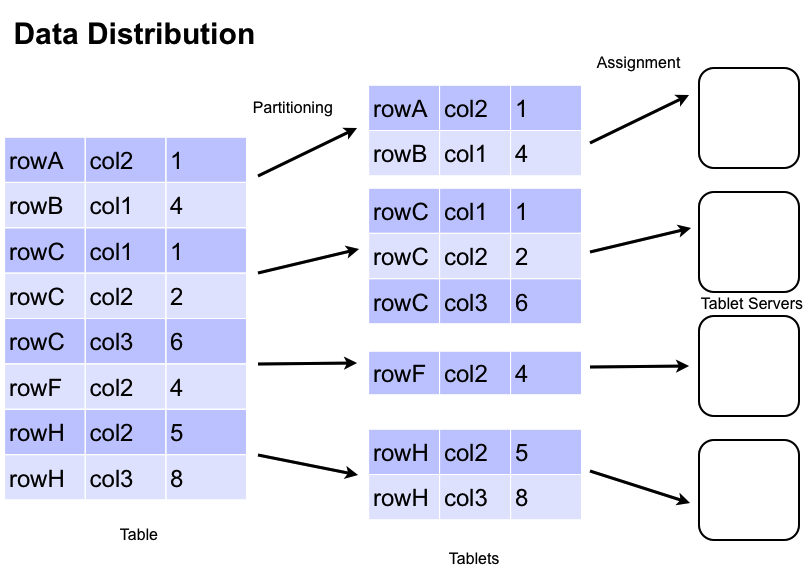
\includegraphics[scale=0.4]{images/data_distribution.png}
\end{center}

\section{Tablet Service}


When a write arrives at a TabletServer it is written to a Write-Ahead Log and
then inserted into a sorted data structure in memory called a MemTable. When the
MemTable reaches a certain size the TabletServer writes out the sorted key-value
pairs to a file in HDFS called Indexed Sequential Access Method (ISAM)
file. This process is called a minor compaction.  A new MemTable is then created
and the fact of the compaction is recorded in the Write-Ahead Log.

When a request to read data arrives at a TabletServer, the TabletServer does a
binary search across the MemTable as well as the in-memory indexes associated
with each ISAM file to find the relevant values. If clients are performing a
scan, several key-value pairs are returned to the client in order from the
MemTable and the set of ISAM files by performing a merge-sort as they are read.

\section{Compactions}

In order to manage the number of files per tablet, periodically the TabletServer
performs Major Compactions of files within a tablet, in which some set of ISAM
files are combined into one file. The previous files will eventually be removed
by the Garbage Collector. This also provides an opportunity to permanently
remove deleted key-value pairs by omitting key-value pairs suppressed by a
delete entry when the new file is created.

\section{Fault-Tolerance}

If a TabletServer fails, the Master detects it and automatically reassigns the tablets
assigned from the failed server to other servers. Any key-value pairs that were in
memory at the time the TabletServer are automatically reapplied from the Write-Ahead
Log to prevent any loss of data.

The Master will coordinate the copying of write-ahead logs to HDFS so the logs
are available to all tablet servers. To make recovery efficient, the updates
within a log are grouped by tablet.  The sorting process can be performed by
Hadoops MapReduce or the Logger server. TabletServers can quickly apply the
mutations from the sorted logs that are destined for the tablets they have now
been assigned.

TabletServer failures are noted on the Master's monitor page, accessible via\\
\mbox{http://master-address:50095/monitor}.

\begin{center}
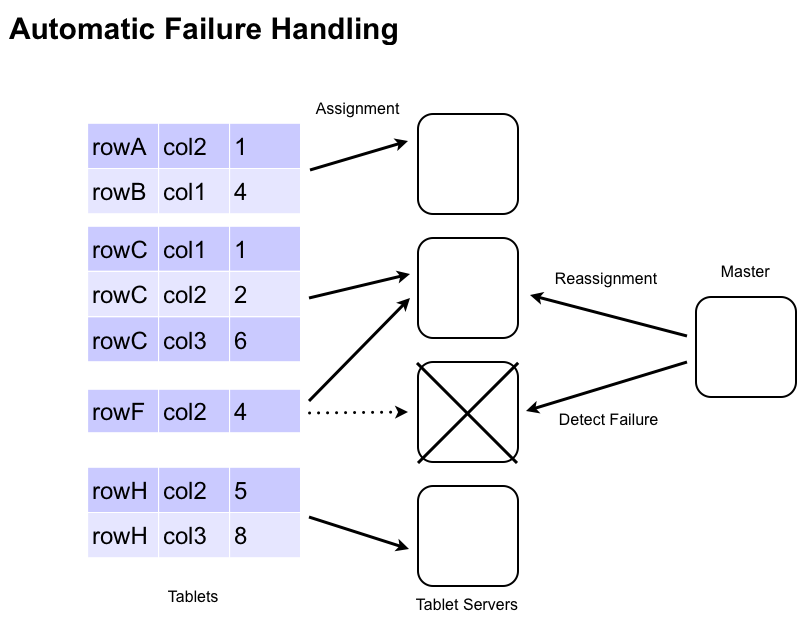
\includegraphics[scale=0.4]{images/failure_handling.png}
\end{center}



% Licensed to the Apache Software Foundation (ASF) under one or more
% contributor license agreements.  See the NOTICE file distributed with
% this work for additional information regarding copyright ownership.
% The ASF licenses this file to You under the Apache License, Version 2.0
% (the "License"); you may not use this file except in compliance with
% the License.  You may obtain a copy of the License at
%
%     http://www.apache.org/licenses/LICENSE-2.0
%
% Unless required by applicable law or agreed to in writing, software
% distributed under the License is distributed on an "AS IS" BASIS,
% WITHOUT WARRANTIES OR CONDITIONS OF ANY KIND, either express or implied.
% See the License for the specific language governing permissions and
% limitations under the License.

\chapter{Accumulo Shell} 
Accumulo provides a simple shell that can be used to examine the contents and
configuration settings of tables, insert/update/delete values, and change
configuration settings.  

The shell can be started by the following command:

\small
\begin{verbatim}
$ACCUMULO_HOME/bin/accumulo shell -u [username]
\end{verbatim}

\normalsize

The shell will prompt for the corresponding password to the username specified
and then display the following prompt:

\small
\begin{verbatim}
Shell - Apache Accumulo Interactive Shell
-
- version 1.3
- instance name: myinstance
- instance id: 00000000-0000-0000-0000-000000000000
-
- type 'help' for a list of available commands
-
\end{verbatim}
\normalsize

\section{Basic Administration}

The Accumulo shell can be used to create and delete tables, as well as to configure
table and instance specific options.

\small
\begin{verbatim}
root@myinstance> tables
!METADATA

root@myinstance> createtable mytable

root@myinstance mytable>

root@myinstance mytable> tables
!METADATA
mytable

root@myinstance mytable> createtable testtable

root@myinstance testtable>

root@myinstance junk> deletetable testtable

root@myinstance>
\end{verbatim}
\normalsize

The Shell can also be used to insert updates and scan tables. This is useful for
inspecting tables.

\small
\begin{verbatim}
root@myinstance mytable> scan

root@myinstance mytable> insert row1 colf colq value1
insert successful

root@myinstance mytable> scan
row1 colf:colq [] value1
\end{verbatim}
\normalsize

The value in brackets "[]" would be the visibility labels.  Since none were used, this is empty for this row.
You can use the "-t" option to scan to see the timestamp for the cell, too.

\section{Table Maintenance}

The \textbf{compact} command instructs Accumulo to schedule a compaction of the table during which
files are consolidated and deleted entries are removed.

\small
\begin{verbatim}
root@myinstance mytable> compact -t mytable
07 16:13:53,201 [shell.Shell] INFO : Compaction of table mytable
scheduled for 20100707161353EDT
\end{verbatim}
\normalsize

The \textbf{flush} command instructs Accumulo to write all entries currently in memory for a given table
to disk.

\small
\begin{verbatim}
root@myinstance mytable> flush -t mytable
07 16:14:19,351 [shell.Shell] INFO : Flush of table mytable
initiated...
\end{verbatim}
\normalsize

\section{User Administration}

The Shell can be used to add, remove, and grant privileges to users.

\small
\begin{verbatim}
root@myinstance mytable> createuser bob
Enter new password for 'bob': *********
Please confirm new password for 'bob': *********

root@myinstance mytable> authenticate bob
Enter current password for 'bob': *********
Valid

root@myinstance mytable> grant System.CREATE_TABLE -s -u bob

root@myinstance mytable> user bob
Enter current password for 'bob': *********

bob@myinstance mytable> userpermissions
System permissions: System.CREATE_TABLE
Table permissions (!METADATA): Table.READ
Table permissions (mytable): NONE

bob@myinstance mytable> createtable bobstable
bob@myinstance bobstable>

bob@myinstance bobstable> user root
Enter current password for 'root': *********

root@myinstance bobstable> revoke System.CREATE_TABLE -s -u bob
\end{verbatim}
\normalsize



% Licensed to the Apache Software Foundation (ASF) under one or more
% contributor license agreements.  See the NOTICE file distributed with
% this work for additional information regarding copyright ownership.
% The ASF licenses this file to You under the Apache License, Version 2.0
% (the "License"); you may not use this file except in compliance with
% the License.  You may obtain a copy of the License at
%
%     http://www.apache.org/licenses/LICENSE-2.0
%
% Unless required by applicable law or agreed to in writing, software
% distributed under the License is distributed on an "AS IS" BASIS,
% WITHOUT WARRANTIES OR CONDITIONS OF ANY KIND, either express or implied.
% See the License for the specific language governing permissions and
% limitations under the License.

\chapter{Writing Accumulo Clients}

\section{Running Client Code}

There are multiple ways to run Java code that uses Accumulo.  Below is a list
of the different ways to execute client code.

\begin{itemize} 
  \item using java executable 
  \item using the accumulo script
  \item using the tool script 
\end{itemize}

Inorder to run client code written to run against Accumulo, you will need to
include the jars that Accumulo depends on in your classpath.  Accumulo client
code depends on Hadoop and Zookeeper.  For Hadoop add the hadoop core jar, all
of the jars in the Hadoop lib directory, and the conf directory to the
classpath. For Zookeeper 3.3 you only need to add the Zookeeper jar, and not
what is in the Zookeeper lib directory.  You can run the following command on a
configured Accumulo system to see what its using for its classpath.

\small 
\begin{verbatim} 
$ACCUMULO_HOME/bin/accumulo classpath 
\end{verbatim}
\normalsize

Another option for running your code is to put a jar file in
\texttt{\$ACCUMULO\_HOME/lib/ext}.  After doing this you can use the accumulo
script to execute your code.  For example if you create a jar containing the
class com.foo.Client and placed that in lib/ext, then you could use the command
\texttt{\$ACCUMULO\_HOME/bin/accumulo com.foo.Client} to execute your code.

If you are writing map reduce job that access Accumulo, then you can use the
bin/tool.sh script to run those jobs.  See the map reduce example.

\section{Connecting}

All clients must first identify the Accumulo instance to which they will be
communicating. Code to do this is as follows:

\small
\begin{verbatim}
String instanceName = "myinstance";
String zooServers = "zooserver-one,zooserver-two"
Instance inst = new ZooKeeperInstance(instanceName, zooServers);

Connector conn = inst.getConnector("user", "passwd");
\end{verbatim}
\normalsize

\section{Writing Data}

Data are written to Accumulo by creating Mutation objects that represent all the
changes to the columns of a single row. The changes are made atomically in the
TabletServer. Clients then add Mutations to a BatchWriter which submits them to
the appropriate TabletServers.

Mutations can be created thus:

\small
\begin{verbatim}
Text rowID = new Text("row1");
Text colFam = new Text("myColFam");
Text colQual = new Text("myColQual");
ColumnVisibility colVis = new ColumnVisibility("public");
long timestamp = System.currentTimeMillis();

Value value = new Value("myValue".getBytes());

Mutation mutation = new Mutation(rowID);
mutation.put(colFam, colQual, colVis, timestamp, value);
\end{verbatim}
\normalsize

\subsection{BatchWriter}
The BatchWriter is highly optimized to send Mutations to multiple TabletServers
and automatically batches Mutations destined for the same TabletServer to
amortize network overhead. Care must be taken to avoid changing the contents of
any Object passed to the BatchWriter since it keeps objects in memory while
batching.

Mutations are added to a BatchWriter thus:

\small
\begin{verbatim}
long memBuf = 1000000L; // bytes to store before sending a batch
long timeout = 1000L; // milliseconds to wait before sending
int numThreads = 10;

BatchWriter writer =
    conn.createBatchWriter("table", memBuf, timeout, numThreads)

writer.add(mutation);

writer.close();
\end{verbatim}
\normalsize

An example of using the batch writer can be found at\\
accumulo/docs/examples/README.batch

\section{Reading Data}

Accumulo is optimized to quickly retrieve the value associated with a given key, and
to efficiently return ranges of consecutive keys and their associated values.

\subsection{Scanner}

To retrieve data, Clients use a Scanner, which provides acts like an Iterator over
keys and values. Scanners can be configured to start and stop at particular keys, and
to return a subset of the columns available.

\small
\begin{verbatim}
// specify which visibilities we are allowed to see
Authorizations auths = new Authorizations("public");

Scanner scan =
    conn.createScanner("table", auths);

scan.setRange(new Range("harry","john"));
scan.fetchFamily("attributes");

for(Entry<Key,Value> entry : scan) {
    String row = e.getKey().getRow();
    Value value = e.getValue();
}
\end{verbatim}
\normalsize

\subsection{Isolated Scanner}

Accumulo supports the ability to present an isolated view of rows when
scanning.  There are three possible ways that a row could change in accumulo :

\begin{itemize}
 \item a mutation applied to a table
 \item iterators executed as part of a minor or major compaction
 \item bulk import of new files
\end{itemize}

Isolation guarantees that either all or none of the changes made by these
operations on a row are seen.  Use the IsolatedScanner to obtain an isolated
view of an accumulo table.  When using the regular scanner it is possible to see
a non isolated view of a row.  For example if a mutation modifies three
columns, it is possible that you will only see two of those modifications.
With the isolated scanner either all three of the changes are seen or none.

The IsolatedScanner buffers rows on the client side so a large row will not
crash a tablet server.  By default rows are buffered in memory, but the user
can easily supply their own buffer if they wish to buffer to disk when rows are
large.

For an example, look at the following\\ 
\texttt{src/examples/src/main/java/org/apache/accumulo/examples/isolation/InterferenceTest.java}

\subsection{BatchScanner}

For some types of access, it is more efficient to retrieve several ranges
simultaneously. This arises when accessing a set of rows that are not consecutive
whose IDs have been retrieved from a secondary index, for example.

The BatchScanner is configured similarly to the Scanner; it can be configured to
retrieve a subset of the columns available, but rather than passing a single Range,
BatchScanners accept a set of Ranges. It is important to note that the keys returned
by a BatchScanner are not in sorted order since the keys streamed are from multiple
TabletServers in parallel.

\small
\begin{verbatim}
ArrayList<Range> ranges = new ArrayList<Range>();
// populate list of ranges ...

BatchScanner bscan =
    conn.createBatchScanner("table", auths, 10);

bscan.setRanges(ranges);
bscan.fetchFamily("attributes");

for(Entry<Key,Value> entry : scan)
    System.out.println(e.getValue());
\end{verbatim}
\normalsize

An example of the BatchScanner can be found at\\
accumulo/docs/examples/README.batch



% Licensed to the Apache Software Foundation (ASF) under one or more
% contributor license agreements.  See the NOTICE file distributed with
% this work for additional information regarding copyright ownership.
% The ASF licenses this file to You under the Apache License, Version 2.0
% (the "License"); you may not use this file except in compliance with
% the License.  You may obtain a copy of the License at
%
%     http://www.apache.org/licenses/LICENSE-2.0
%
% Unless required by applicable law or agreed to in writing, software
% distributed under the License is distributed on an "AS IS" BASIS,
% WITHOUT WARRANTIES OR CONDITIONS OF ANY KIND, either express or implied.
% See the License for the specific language governing permissions and
% limitations under the License.

\chapter{Table Configuration}

Accumulo tables have a few options that can be configured to alter the default
behavior of Accumulo as well as improve performance based on the data stored.
These include locality groups, constraints, bloom filters, iterators, and block cache.

\section{Locality Groups}
Accumulo supports storing of sets of column families separately on disk to allow
clients to scan over columns that are frequently used together efficient and to avoid
scanning over column families that are not requested. After a locality group is set
Scanner and BatchScanner operations will automatically take advantage of them
whenever the fetchColumnFamilies() method is used.

By default tables place all column families into the same ``default" locality group.
Additional locality groups can be configured anytime via the shell or
programmatically as follows:

\subsection{Managing Locality Groups via the Shell}

\small
\begin{verbatim}
usage: setgroups <group>=<col fam>{,<col fam>}{ <group>=<col fam>{,<col
fam>}} [-?] -t <table>

user@myinstance mytable> setgroups -t mytable group_one=colf1,colf2

user@myinstance mytable> getgroups -t mytable
group_one=colf1,colf2
\end{verbatim}
\normalsize

\subsection{Managing Locality Groups via the Client API}

\small
\begin{verbatim}
Connector conn;

HashMap<String,Set<Text>> localityGroups =
    new HashMap<String, Set<Text>>();

HashSet<Text> metadataColumns = new HashSet<Text>();
metadataColumns.add(new Text("domain"));
metadataColumns.add(new Text("link"));

HashSet<Text> contentColumns = new HashSet<Text>();
contentColumns.add(new Text("body"));
contentColumns.add(new Text("images"));

localityGroups.put("metadata", metadataColumns);
localityGroups.put("content", contentColumns);

conn.tableOperations().setLocalityGroups("mytable", localityGroups);

// existing locality groups can be obtained as follows
Map<String, Set<Text>> groups =
    conn.tableOperations().getLocalityGroups("mytable");
\end{verbatim}
\normalsize

The assignment of Column Families to Locality Groups can be changed anytime. The
physical movement of column families into their new locality groups takes place via
the periodic Major Compaction process that takes place continuously in the
background. Major Compaction can also be scheduled to take place immediately
through the shell:

\small
\begin{verbatim}
user@myinstance mytable> compact -t mytable
\end{verbatim}
\normalsize

\section{Constraints}

Accumulo supports constraints applied on mutations at insert time. This can be
used to disallow certain inserts according to a user defined policy. Any mutation
that fails to meet the requirements of the constraint is rejected and sent back to the
client.

Constraints can be enabled by setting a table property as follows:

\small
\begin{verbatim}
user@myinstance mytable> config -t mytable -s table.constraint.1=com.test.ExampleConstraint
user@myinstance mytable> config -t mytable -s table.constraint.2=com.test.AnotherConstraint
user@myinstance mytable> config -t mytable -f constraint
---------+--------------------------------+----------------------------
SCOPE    | NAME                           | VALUE
---------+--------------------------------+----------------------------
table    | table.constraint.1............ | com.test.ExampleConstraint
table    | table.constraint.2............ | com.test.AnotherConstraint
---------+--------------------------------+----------------------------
\end{verbatim}
\normalsize

Currently there are no general-purpose constraints provided with the Accumulo
distribution. New constraints can be created by writing a Java class that implements
the org.apache.accumulo.core.constraints.Constraint interface.

To deploy a new constraint, create a jar file containing the class implementing the
new constraint and place it in the lib directory of the Accumulo installation. New
constraint jars can be added to Accumulo and enabled without restarting but any
change to an existing constraint class requires Accumulo to be restarted.

An example of constraints can be found in\\
\texttt{accumulo/docs/examples/README.constraints} with corresponding code under\\
\texttt{accumulo/src/examples/simple/main/java/accumulo/examples/simple/constraints} .

\section{Bloom Filters}
As mutations are applied to an Accumulo table, several files are created per tablet. If
bloom filters are enabled, Accumulo will create and load a small data structure into
memory to determine whether a file contains a given key before opening the file.
This can speed up lookups considerably.

To enable bloom filters, enter the following command in the Shell:

\small
\begin{verbatim}
user@myinstance> config -t mytable -s table.bloom.enabled=true
\end{verbatim}
\normalsize

An extensive example of using Bloom Filters can be found at\\
\texttt{accumulo/docs/examples/README.bloom} .

\section{Iterators}
Iterators provide a modular mechanism for adding functionality to be executed by
TabletServers when scanning or compacting data. This allows users to efficiently
summarize, filter, and aggregate data. In fact, the built-in features of cell-level
security and column fetching are implemented using Iterators.
Some useful Iterators are provided with Accumulo and can be found in the org.apache.accumulo.core.iterators.user package.

\subsection{Setting Iterators via the Shell}

\small
\begin{verbatim}
usage: setiter [-?] -ageoff | -agg | -class <name> | -regex | 
-reqvis | -vers   [-majc] [-minc] [-n <itername>] -p <pri>   
[-scan] [-t <table>]

user@myinstance mytable> setiter -t mytable -scan -p 10 -n myiter
\end{verbatim}
\normalsize

\subsection{Setting Iterators Programmatically}

\small
\begin{verbatim}
scanner.addIterator(new IteratorSetting(
    15, // priority
    "com.company.MyIterator", // class name
    "myiter" // name this iterator
));
\end{verbatim}
\normalsize

Some iterators take additional parameters from client code, as in the following
example:

\small
\begin{verbatim}
IteratorSetting iter = new IteratorSetting(...);
iter.addOption("myoptionname", "myoptionvalue");
scanner.addIterator(iter)
\end{verbatim}
\normalsize

Tables support separate Iterator settings to be applied at scan time, upon minor
compaction and upon major compaction. For most uses, tables will have identical
iterator settings for all three to avoid inconsistent results.

\subsection{Versioning Iterators and Timestamps}

Accumulo provides the capability to manage versioned data through the use of
timestamps within the Key. If a timestamp is not specified in the key created by the
client then the system will set the timestamp to the current time. Two keys with
identical rowIDs and columns but different timestamps are considered two versions
of the same key. If two inserts are made into accumulo with the same rowID,
column, and timestamp, then the behavior is non-deterministic.

Timestamps are sorted in descending order, so the most recent data comes first.
Accumulo can be configured to return the top k versions, or versions later than a
given date. The default is to return the one most recent version.

The version policy can be changed by changing the VersioningIterator options for a
table as follows:

\small
\begin{verbatim}
user@myinstance mytable> config -t mytable -s
table.iterator.scan.vers.opt.maxVersions=3

user@myinstance mytable> config -t mytable -s
table.iterator.minc.vers.opt.maxVersions=3

user@myinstance mytable> config -t mytable -s
table.iterator.majc.vers.opt.maxVersions=3
\end{verbatim}
\normalsize

\subsubsection{Logical Time}

Accumulo 1.2 introduces the concept of logical time. This ensures that timestamps
set by accumulo always move forward. This helps avoid problems caused by
TabletServers that have different time settings. The per tablet counter gives unique
one up time stamps on a per mutation basis. When using time in milliseconds, if
two things arrive within the same millisecond then both receive the same
timestamp.  When using time in milliseconds, accumulo set times will still
always move forward and never backwards.

A table can be configured to use logical timestamps at creation time as follows:

\small
\begin{verbatim}
user@myinstance> createtable -tl logical
\end{verbatim}
\normalsize

\subsubsection{Deletes}
Deletes are special keys in accumulo that get sorted along will all the other data.
When a delete key is inserted, accumulo will not show anything that has a
timestamp less than or equal to the delete key. During major compaction, any keys
older than a delete key are omitted from the new file created, and the omitted keys
are removed from disk as part of the regular garbage collection process.

\subsection{Filters}
When scanning over a set of key-value pairs it is possible to apply an arbitrary
filtering policy through the use of a Filter. Filters are types of iterators that return
only key-value pairs that satisfy the filter logic. Accumulo has a few built-in filters
that can be configured on any table: AgeOff, ColumnAgeOff, Timestamp, NoVis, and RegEx. More can be added
by writing a Java class that extends the\\
org.apache.accumulo.core.iterators.Filter class.

The AgeOff filter can be configured to remove data older than a certain date or a fixed
amount of time from the present. The following example sets a table to delete
everything inserted over 30 seconds ago:

\small
\begin{verbatim}
user@myinstance> createtable filtertest
user@myinstance filtertest> setiter -t filtertest -scan -minc -majc -p 10 -n myfilter -ageoff
AgeOffFilter removes entries with timestamps more than <ttl> milliseconds old
----------> set org.apache.accumulo.core.iterators.user.AgeOffFilter parameter negate, default false keeps k/v that pass accept method, true rejects k/v that pass accept method: 
----------> set org.apache.accumulo.core.iterators.user.AgeOffFilter parameter ttl, time to live (milliseconds): 3000
----------> set org.apache.accumulo.core.iterators.user.AgeOffFilter parameter currentTime, if set, use the given value as the absolute time in milliseconds as the current time of day: 
user@myinstance filtertest> 
user@myinstance filtertest> scan
user@myinstance filtertest> insert foo a b c
user@myinstance filtertest> scan
foo a:b [] c
user@myinstance filtertest> sleep 4
user@myinstance filtertest> scan
user@myinstance filtertest>
\end{verbatim}
\normalsize

To see the iterator settings for a table, use:

\small
\begin{verbatim}
user@example filtertest> config -t filtertest -f iterator
---------+---------------------------------------------+------------------
SCOPE    | NAME                                        | VALUE
---------+---------------------------------------------+------------------
table    | table.iterator.majc.myfilter .............. | 10,org.apache.accumulo.core.iterators.user.AgeOffFilter
table    | table.iterator.majc.myfilter.opt.ttl ...... | 3000
table    | table.iterator.majc.vers .................. | 20,org.apache.accumulo.core.iterators.VersioningIterator
table    | table.iterator.majc.vers.opt.maxVersions .. | 1
table    | table.iterator.minc.myfilter .............. | 10,org.apache.accumulo.core.iterators.user.AgeOffFilter
table    | table.iterator.minc.myfilter.opt.ttl ...... | 3000
table    | table.iterator.minc.vers .................. | 20,org.apache.accumulo.core.iterators.VersioningIterator
table    | table.iterator.minc.vers.opt.maxVersions .. | 1
table    | table.iterator.scan.myfilter .............. | 10,org.apache.accumulo.core.iterators.user.AgeOffFilter
table    | table.iterator.scan.myfilter.opt.ttl ...... | 3000
table    | table.iterator.scan.vers .................. | 20,org.apache.accumulo.core.iterators.VersioningIterator
table    | table.iterator.scan.vers.opt.maxVersions .. | 1
---------+------------------------------------------+------------------
\end{verbatim}
\normalsize

\subsection{Combiners}

Accumulo allows Combiners to be configured on tables and column
families. When a Combiner is set it is applied across the values
associated with any keys that share rowID, column family, and column qualifier.
This is similar to the reduce step in MapReduce, which applied some function to all
the values associated with a particular key.

For example, if a summing combiner were configured on a table and the following
mutations were inserted:

\small
\begin{verbatim}
Row     Family Qualifier Timestamp  Value
rowID1  colfA  colqA     20100101   1
rowID1  colfA  colqA     20100102   1
\end{verbatim}
\normalsize

The table would reflect only one aggregate value:

\small
\begin{verbatim}
rowID1  colfA  colqA     -          2
\end{verbatim}
\normalsize

Combiners can be enabled for a table using the setiter command in the shell.  Below is an example.

\small
\begin{verbatim}
root@a14 perDayCounts> setiter -t perDayCounts -p 10 -scan -minc -majc -n daycount 
                       -class org.apache.accumulo.core.iterators.user.SummingCombiner
TypedValueCombiner can interpret Values as a variety of number encodings 
  (VLong, Long, or String) before combining
----------> set SummingCombiner parameter columns, 
            <col fam>[:<col qual>]{,<col fam>[:<col qual>]} : day
----------> set SummingCombiner parameter type, <VARNUM|LONG|STRING>: STRING

root@a14 perDayCounts> insert foo day 20080101 1
root@a14 perDayCounts> insert foo day 20080101 1
root@a14 perDayCounts> insert foo day 20080103 1
root@a14 perDayCounts> insert bar day 20080101 1
root@a14 perDayCounts> insert bar day 20080101 1

root@a14 perDayCounts> scan
bar day:20080101 []    2
foo day:20080101 []    2
foo day:20080103 []    1
\end{verbatim}
\normalsize

Accumulo includes some useful Combiners out of the box.  To find these look in
the\\ \textbf{org.apache.accumulo.core.iterators.user} package.

Additional Combiners can be added by creating a Java class that extends\\
\textbf{org.apache.accumulo.core.iterators.Combiner} and adding a jar containing that
class to Accumulo's lib/ext directory.

An example of a Combiner can be found under\\
accumulo/src/examples/simple/main/java/org/apache/accumulo/examples/simple/combiner/StatsCombiner.java


\section{Block Cache}

In order to increase throughput of commonly accessed entries, Accumulo employs a block cache.
This block cache buffers data in memory so that it doesn't have to be read off of disk.
The RFile format that Accumulo prefers is a mix of index blocks and data blocks, where the index blocks are used to find the appropriate data blocks.
Typical queries to Accumulo result in a binary search over several index blocks followed by a linear scan of one or more data blocks.

The block cache can be configured on a per-table basis, and all tablets hosted on a tablet server share a single resource pool.
To configure the size of the tablet server's block cache, set the following properties:
\begin{verbatim}
tserver.cache.data.size: Specifies the size of the cache for file data blocks.
tserver.cache.index.size: Specifies the size of the cache for file indices.
\end{verbatim}
To enable the block cache for your table, set the following properties:
\begin{verbatim}
table.cache.block.enable: Determines whether file (data) block cache is enabled.
table.cache.index.enable: Determines whether index cache is enabled.
\end{verbatim}

The block cache can have a significant effect on alleviating hot spots, as well as reducing query latency.
It is enabled by default for the !METADATA table.

\section{Compaction}

As data is written to Accumulo it is buffered in memory.  The data buffered in
memory is eventually written to HDFS on a per tablet basis.  Files can also be
added to tablets directly by bulk import.  In the background tablet servers run
major compactions to merge multiple files into one.  The tablet server has to
decide which tablets to compact and which files within a tablet to compact.
This decision is made using the compaction ratio, which is configurable on a
per table basis.  To configure this ratio modify the following property:

\begin{verbatim}
table.compaction.major.ratio
\end{verbatim}  

Increasing this ratio will result in more files per tablet and less compaction
work.  More files per tablet means more higher query latency.  So adjusting
this ratio is a trade off between ingest and query performance.  The ratio
defaults to 3.  

The way the ratio works is that a set of files is compacted into one file if the
sum of the sizes of the files in the set is larger than the ratio multiplied by
the size of the largest file in the set. If this is not true for the set of all
files in a tablet, the largest file is removed from consideration, and the
remaining files are considered for compaction. This is repeated until a
compaction is triggered or there are no files left to consider.

The number of background threads tablet servers use to run major compactions is
configurable.  To configure this modify the following property:

\begin{verbatim}
tserver.compaction.major.concurrent.max
\end{verbatim}

Also, the number of threads tablet servers use for minor compactions is
configurable.  To configure this modify the following property:

\begin{verbatim}
tserver.compaction.minor.concurrent.max
\end{verbatim}

The numbers of minor and major compactions running and queued is visible on the
Accumulo monitor page.  This allows you to see if compactions are backing up
and adjustments to the above settings are needed.  When adjusting the number of
threads available for compactions, consider the number of cores and other tasks
running on the nodes such as maps and reduces.

If major compactions are not keeping up, then the number of files per tablet
will grow to a point such that query performance starts to suffer. One way to
handle this situation is to increase the compaction ratio.  For example, if the
compaction ratio were set to 1, then every new file added to a tablet by minor
compaction would immediately queue the tablet for major compaction. So if a
tablet has a 200M file and minor compaction writes a 1M file, then the major
compaction will attempt to merge the 200M and 1M file.  If the tablet server
has lots of tablets trying to do this sort of thing, then major compactions
will back up and the number of files per tablet will start to grow, assuming
data is being continuously written.  Increasing the compaction ratio will
alleviate backups by lowering the amount of major compaction work that needs to
be done.

Another option to deal with the files per tablet growing too large is to adjust
the following property:

\begin{verbatim}
table.file.max  
\end{verbatim}

When a tablet reaches this number of files and needs to flush its in-memory
data to disk, it will choose to do a merging minor compaction.  A merging minor
compaction will merge the tablet's smallest file with the data in memory at
minor compaction time.  Therefore the number of files will not grow beyond this
limit.  This will make minor compactions take longer, which will cause ingest
performance to decrease.  This can cause ingest to slow down until major
compactions have enough time to catch up.   When adjusting this property, also
consider adjusting the compaction ratio. Ideally, merging minor compactions
never need to occur and major compactions will keep up. It is possible to
configure the file max and compaction ratio such that only merging minor
compactions occur and major compactions never occur. This should be avoided
because doing only merging minor compactions causes $O(N^2)$ work to be done.
The amount of work done by major compactions is $O(N*\log_R(N))$ where
\textit{R} is the compaction ratio.

Compactions can be initiated manually for a table.  To initiate a minor
compaction, use the flush command in the shell.  To initiate a major compaction,
use the compact command in the shell.  The compact command will compact all
tablets in a table to one file.  Even tablets with one file are compacted.  This
is useful for the case where a major compaction filter is configured for a
table. In 1.4 the ability to compact a range of a table was added.  To use this
feature specify start and stop rows for the compact command.  This will only
compact tablets that overlap the given row range.

\section{Pre-splitting tables}

Accumulo will balance and distribute tables accross servers. Before a
table gets large, it will be maintained as a single tablet on a single
server.  This limits the speed at which data can be added or queried
to the speed of a single node. To improve performance when the a table
is new, or small, you can add split points and generate new tablets.

In the shell:

\small
\begin{verbatim}
root@myinstance> createtable newTable
root@myinstance> addsplits -t newTable g n t
\end{verbatim}
\normalsize

This will create a new table with 4 tablets.  The table will be split
on the letters ``g'', ``n'', and ``t'' which will work nicely if the
row data start with lower-case alphabetic characters.  If your row
data includes binary information or numeric information, or if the
distribution of the row information is not flat, then you would pick
different split points.  Now ingest and query can proceed on 4 nodes
which can improve performance.

\section{Merging tablets}

Over time, a table can get very large, so large that it has hundreds
of thousands of split points.  Once there are enough tablets to spread
a table across the entire cluster, additional splits may not improve
performance, and may create unnecessary bookkeeping.  The distribution
of data may change over time.  For example, if row data contains date
information, and data is continually added and removed to maintain a
window of current information, tablets for older rows may be empty.

Accumulo supports tablet merging, which can be used to reduce delete
the number of split points.  The following command will merge all rows
from ``A'' to ``Z'' into a single tablet:

\small
\begin{verbatim}
root@myinstance> merge -t myTable -s A -e Z
\end{verbatim}
\normalsize

If the result of a merge produces a tablet that is larger than the
configured split size, the tablet may be split by the tablet server.
Be sure to increase your tablet size prior to any merges if the goal
is to have larger tablets:

\small
\begin{verbatim}
root@myinstance> config -t myTable -s table.split.threshold=2G
\end{verbatim}
\normalsize

In order to merge small tablets, you can ask accumulo to merge
sections of a table smaller than a given size.

\small
\begin{verbatim}
root@myinstance> merge -t myTable -s 100M
\end{verbatim}
\normalsize

By default, small tablets will not be merged into tablets that are
already larger than the given size.  This can leave isolated small
tablets.  To force small tablets to be merged into larger tablets use
the ``--force'' option:

\small
\begin{verbatim}
root@myinstance> merge -t myTable -s 100M --force
\end{verbatim}
\normalsize

Merging away small tablets works on one section at a time.  If your
table contains many sections of small split points, or you are
attempting to change the split size of the entire table, it will be
faster to set the split point and merge the entire table:

\small
\begin{verbatim}
root@myinstance> config -t myTable -s table.split.threshold=256M
root@myinstance> merge -t myTable
\end{verbatim}
\normalsize

\section{Delete Range}

Consider an indexing scheme that uses date information in each row.
For example ``20110823-15:20:25.013'' might be a row that specifies a
date and time.  In some cases, we might like to delete rows based on
this date, say to remove all the data older than the current year.
Accumulo supports a delete range operation which can efficiently
removes data between two rows.  For example:

\small
\begin{verbatim}
root@myinstance> deleterange -t myTable -s 2010 -e 2011
\end{verbatim}
\normalsize

This will delete all rows starting with ``2010'' and it will stop at
any row starting ``2011''.  You can delete any data prior to 2011
with:

\small
\begin{verbatim}
root@myinstance> deleterange -t myTable -e 2011 --force
\end{verbatim}
\normalsize

The shell will not allow you to delete an unbounded range (no start)
unless you provide the ``--force'' option.

Range deletion is implemented using splits at the given start/end
positions, and will affect the number of splits in the table.

\section{Cloning Tables}

A new table can be created that points to an existing table's data.  This is a
very quick metadata operation, no data is actually copied.  The cloned table
and the source table can change independently after the clone operation.  One
use case for this feature is testing.  For example to test a new filtering
iterator, clone the table, add the filter to the clone, and force a major
compaction.  To perform a test on less data, clone a table and then use delete
range to efficiently remove a lot of data from the clone.  Another use case is
generating a snapshot to guard against human error.  To create a snapshot,
clone a table and then disable write permissions on the clone.

The clone operation will point to the source table's files.  This is why the
flush option is present and is enabled by default in the shell.  If the flush
option is not enabled, then any data the source table currently has in memory
will not exist in the clone.

A cloned table copies the configuration of the source table.  However the
permissions of the source table are not copied to the clone.  After a clone is
created, only the user that created the clone can read and write to it.

In the following example we see that data inserted after the clone operation is
not visible in the clone.

\small
\begin{verbatim}
root@a14> createtable people
root@a14 people> insert 890435 name last Doe
root@a14 people> insert 890435 name first John
root@a14 people> clonetable people test  
root@a14 people> insert 890436 name first Jane
root@a14 people> insert 890436 name last Doe  
root@a14 people> scan
890435 name:first []    John
890435 name:last []    Doe
890436 name:first []    Jane
890436 name:last []    Doe
root@a14 people> table test
root@a14 test> scan
890435 name:first []    John
890435 name:last []    Doe
root@a14 test> 
\end{verbatim}
\normalsize

The du command in the shell shows how much space a table is using in HDFS.
This command can also show how much overlapping space two cloned tables have in
HDFS.  In the example below du shows table ci is using 428M.  Then ci is cloned
to cic and du shows that both tables share 428M.  After three entries are
inserted into cic and its flushed, du shows the two tables still share 428M but
cic has 226 bytes to itself.  Finally, table cic is compacted and then du shows
that each table uses 428M.

\small
\begin{verbatim}
root@a14> du ci           
             428,482,573 [ci]
root@a14> clonetable ci cic
root@a14> du ci cic
             428,482,573 [ci, cic]
root@a14> table cic
root@a14 cic> insert r1 cf1 cq1 v1
root@a14 cic> insert r1 cf1 cq2 v2
root@a14 cic> insert r1 cf1 cq3 v3 
root@a14 cic> flush -t cic -w 
27 15:00:13,908 [shell.Shell] INFO : Flush of table cic completed.
root@a14 cic> du ci cic       
             428,482,573 [ci, cic]
                     226 [cic]
root@a14 cic> compact -t cic -w
27 15:00:35,871 [shell.Shell] INFO : Compacting table ...
27 15:03:03,303 [shell.Shell] INFO : Compaction of table cic completed for given range
root@a14 cic> du ci cic        
             428,482,573 [ci]
             428,482,612 [cic]
root@a14 cic> 
\end{verbatim}
\normalsize

\section{Exporting Tables}

Accumulo supports exporting tables for the purpose of copying tables to another
cluster.  Exporting and importing tables preserves the tables configuration,
splits, and logical time.  Tables are exported and then copied via the hadoop
distcp command.  To export a table, it must be offline and stay offline while
discp runs.  The reason it needs to stay offline is to prevent files from being
deleted.  A table can be cloned and the clone taken offline inorder to avoid
losing access to the table.  See docs/examples/README.example for an example.


% Licensed to the Apache Software Foundation (ASF) under one or more
% contributor license agreements.  See the NOTICE file distributed with
% this work for additional information regarding copyright ownership.
% The ASF licenses this file to You under the Apache License, Version 2.0
% (the "License"); you may not use this file except in compliance with
% the License.  You may obtain a copy of the License at
%
%     http://www.apache.org/licenses/LICENSE-2.0
%
% Unless required by applicable law or agreed to in writing, software
% distributed under the License is distributed on an "AS IS" BASIS,
% WITHOUT WARRANTIES OR CONDITIONS OF ANY KIND, either express or implied.
% See the License for the specific language governing permissions and
% limitations under the License.

\chapter{Table Design}

\section{Basic Table}

Since Accumulo tables are sorted by row ID, each table can be thought of as being
indexed by the row ID. Lookups performed row ID can be executed quickly, by doing
a binary search, first across the tablets, and then within a tablet. Clients should
choose a row ID carefully in order to support their desired application. A simple rule
is to select a unique identifier as the row ID for each entity to be stored and assign
all the other attributes to be tracked to be columns under this row ID. For example,
if we have the following data in a comma-separated file:

\small
\begin{verbatim}
    userid,age,address,account-balance
\end{verbatim}
\normalsize

We might choose to store this data using the userid as the rowID and the rest of the
data in column families:

\small
\begin{verbatim}
Mutation m = new Mutation(new Text(userid));
m.put(new Text("age"), age);
m.put(new Text("address"), address);
m.put(new Text("balance"), account_balance);

writer.add(m);
\end{verbatim}
\normalsize

We could then retrieve any of the columns for a specific userid by specifying the
userid as the range of a scanner and fetching specific columns:

\small
\begin{verbatim}
Range r = new Range(userid, userid); // single row
Scanner s = conn.createScanner("userdata", auths);
s.setRange(r);
s.fetchColumnFamily(new Text("age"));

for(Entry<Key,Value> entry : s)
    System.out.println(entry.getValue().toString());
\end{verbatim}
\normalsize

\section{RowID Design}

Often it is necessary to transform the rowID in order to have rows ordered in a way
that is optimal for anticipated access patterns. A good example of this is reversing
the order of components of internet domain names in order to group rows of the
same parent domain together:

\small
\begin{verbatim}
com.google.code
com.google.labs
com.google.mail
com.yahoo.mail
com.yahoo.research
\end{verbatim}
\normalsize

Some data may result in the creation of very large rows - rows with many columns.
In this case the table designer may wish to split up these rows for better load
balancing while keeping them sorted together for scanning purposes. This can be
done by appending a random substring at the end of the row:

\small
\begin{verbatim}
com.google.code_00
com.google.code_01
com.google.code_02
com.google.labs_00
com.google.mail_00
com.google.mail_01
\end{verbatim}
\normalsize

It could also be done by adding a string representation of some period of time such as date to the week
or month:

\small
\begin{verbatim}
com.google.code_201003
com.google.code_201004
com.google.code_201005
com.google.labs_201003
com.google.mail_201003
com.google.mail_201004
\end{verbatim}
\normalsize

Appending dates provides the additional capability of restricting a scan to a given
date range.

\section{Indexing}
In order to support lookups via more than one attribute of an entity, additional
indexes can be built. However, because Accumulo tables can support any number of
columns without specifying them beforehand, a single additional index will often
suffice for supporting lookups of records in the main table. Here, the index has, as
the rowID, the Value or Term from the main table, the column families are the same,
and the column qualifier of the index table contains the rowID from the main table.

\begin{center}
$\begin{array}{|c|c|c|c|c|c|} \hline
\multicolumn{5}{|c|}{\mbox{Key}} & \multirow{3}{*}{\mbox{Value}}\\ \cline{1-5}
\multirow{2}{*}{\mbox{Row ID}}& \multicolumn{3}{|c|}{\mbox{Column}} & \multirow{2}{*}{\mbox{Timestamp}} & \\ \cline{2-4}
& \mbox{Family} & \mbox{Qualifier} & \mbox{Visibility} & & \\ \hline \hline
\mbox{Term} & \mbox{Field Name} & \mbox{MainRowID} & & &\\ \hline
\end{array}$
\end{center}

Note: We store rowIDs in the column qualifier rather than the Value so that we can
have more than one rowID associated with a particular term within the index. If we
stored this in the Value we would only see one of the rows in which the value
appears since Accumulo is configured by default to return the one most recent
value associated with a key.

Lookups can then be done by scanning the Index Table first for occurrences of the
desired values in the columns specified, which returns a list of row ID from the main
table. These can then be used to retrieve each matching record, in their entirety, or a
subset of their columns, from the Main Table.

To support efficient lookups of multiple rowIDs from the same table, the Accumulo
client library provides a BatchScanner. Users specify a set of Ranges to the
BatchScanner, which performs the lookups in multiple threads to multiple servers
and returns an Iterator over all the rows retrieved. The rows returned are NOT in
sorted order, as is the case with the basic Scanner interface.

\small
\begin{verbatim}
// first we scan the index for IDs of rows matching our query

Text term = new Text("mySearchTerm");

HashSet<Text> matchingRows = new HashSet<Text>();

Scanner indexScanner = createScanner("index", auths);
indexScanner.setRange(new Range(term, term));

// we retrieve the matching rowIDs and create a set of ranges
for(Entry<Key,Value> entry : indexScanner)
    matchingRows.add(new Text(entry.getKey().getColumnQualifier()));

// now we pass the set of rowIDs to the batch scanner to retrieve them
BatchScanner bscan = conn.createBatchScanner("table", auths, 10);

bscan.setRanges(matchingRows);
bscan.fetchFamily("attributes");

for(Entry<Key,Value> entry : scan)
    System.out.println(entry.getValue());
\end{verbatim}
\normalsize

One advantage of the dynamic schema capabilities of Accumulo is that different
fields may be indexed into the same physical table. However, it may be necessary to
create different index tables if the terms must be formatted differently in order to
maintain proper sort order. For example, real numbers must be formatted
differently than their usual notation in order to be sorted correctly. In these cases,
usually one index per unique data type will suffice.

\section{Entity-Attribute and Graph Tables}

Accumulo is ideal for storing entities and their attributes, especially of the
attributes are sparse. It is often useful to join several datasets together on common
entities within the same table. This can allow for the representation of graphs,
including nodes, their attributes, and connections to other nodes.

Rather than storing individual events, Entity-Attribute or Graph tables store
aggregate information about the entities involved in the events and the
relationships between entities. This is often preferrable when single events aren't
very useful and when a continuously updated summarization is desired.

The physical schema for an entity-attribute or graph table is as follows:

\begin{center}
$\begin{array}{|c|c|c|c|c|c|} \hline
\multicolumn{5}{|c|}{\mbox{Key}} & \multirow{3}{*}{\mbox{Value}}\\ \cline{1-5}
\multirow{2}{*}{\mbox{Row ID}}& \multicolumn{3}{|c|}{\mbox{Column}} & \multirow{2}{*}{\mbox{Timestamp}} & \\ \cline{2-4}
& \mbox{Family} & \mbox{Qualifier} & \mbox{Visibility} & & \\ \hline \hline
\mbox{EntityID} & \mbox{Attribute Name} & \mbox{Attribute Value} & & & \mbox{Weight} \\ \hline
\mbox{EntityID} & \mbox{Edge Type} & \mbox{Related EntityID} & & & \mbox{Weight} \\ \hline
\end{array}$
\end{center}

For example, to keep track of employees, managers and products the following
entity-attribute table could be used. Note that the weights are not always necessary
and are set to 0 when not used.

$\begin{array}{llll}
\bf{RowID} & \bf{Column Family} & \bf{Column Qualifier} & \bf{Value} \\
\\
E001 & name & bob & 0 \\
E001 & department & sales & 0 \\
E001 & hire\_date & 20030102 & 0 \\
E001 & units\_sold & P001 & 780 \\
\\
E002 & name & george & 0 \\
E002 & department & sales & 0 \\
E002 & manager\_of & E001 & 0 \\
E002 & manager\_of & E003 & 0 \\
\\
E003 & name & harry & 0 \\
E003 & department & accounts\_recv & 0 \\
E003 & hire\_date & 20000405 & 0 \\
E003 & units\_sold & P002 & 566 \\
E003 & units\_sold & P001 & 232 \\
\\
P001 & product\_name & nike\_airs & 0 \\
P001 & product\_type & shoe & 0 \\
P001 & in\_stock & germany & 900 \\
P001 & in\_stock & brazil & 200 \\
\\
P002 & product\_name & basic\_jacket & 0 \\
P002 & product\_type & clothing & 0 \\
P002 & in\_stock & usa & 3454 \\
P002 & in\_stock & germany & 700 \\
\end{array}$
\vspace{5mm}

To allow efficient updating of edge weights, an aggregating iterator can be
configured to add the value of all mutations applied with the same key. These types
of tables can easily be created from raw events by simply extracting the entities,
attributes, and relationships from individual events and inserting the keys into
Accumulo each with a count of 1. The aggregating iterator will take care of
maintaining the edge weights.

\section{Document-Partitioned Indexing}

Using a simple index as described above works well when looking for records that
match one of a set of given criteria. When looking for records that match more than
one criterion simultaneously, such as when looking for documents that contain all of
the words `the' and `white' and `house', there are several issues.

First is that the set of all records matching any one of the search terms must be sent
to the client, which incurs a lot of network traffic. The second problem is that the
client is responsible for performing set intersection on the sets of records returned
to eliminate all but the records matching all search terms. The memory of the client
may easily be overwhelmed during this operation.

For these reasons Accumulo includes support for a scheme known as sharded
indexing, in which these set operations can be performed at the TabletServers and
decisions about which records to include in the result set can be made without
incurring network traffic.

This is accomplished via partitioning records into bins that each reside on at most
one TabletServer, and then creating an index of terms per record within each bin as
follows:

\begin{center}
$\begin{array}{|c|c|c|c|c|c|} \hline
\multicolumn{5}{|c|}{\mbox{Key}} & \multirow{3}{*}{\mbox{Value}}\\ \cline{1-5}
\multirow{2}{*}{\mbox{Row ID}}& \multicolumn{3}{|c|}{\mbox{Column}} & \multirow{2}{*}{\mbox{Timestamp}} & \\ \cline{2-4}
& \mbox{Family} & \mbox{Qualifier} & \mbox{Visibility} & & \\ \hline \hline
\mbox{BinID} & \mbox{Term} & \mbox{DocID} & & & \mbox{Weight} \\ \hline
\end{array}$
\end{center}

Documents or records are mapped into bins by a user-defined ingest application. By
storing the BinID as the RowID we ensure that all the information for a particular
bin is contained in a single tablet and hosted on a single TabletServer since
Accumulo never splits rows across tablets. Storing the Terms as column families
serves to enable fast lookups of all the documents within this bin that contain the
given term.

Finally, we perform set intersection operations on the TabletServer via a special
iterator called the Intersecting Iterator. Since documents are partitioned into many
bins, a search of all documents must search every bin. We can use the BatchScanner
to scan all bins in parallel. The Intersecting Iterator should be enabled on a
BatchScanner within user query code as follows:

\small
\begin{verbatim}
Text[] terms = {new Text("the"), new Text("white"), new Text("house")};

BatchScanner bs = conn.createBatchScanner(table, auths, 20);
IteratorSetting iter = new IteratorSetting(20, "ii", IntersectingIterator.class);
IntersectingIterator.setColumnFamilies(iter, terms);
bs.addScanIterator(iter);
bs.setRanges(Collections.singleton(new Range()));

for(Entry<Key,Value> entry : bs) {
    System.out.println(" " + entry.getKey().getColumnQualifier());
}
\end{verbatim}
\normalsize

This code effectively has the BatchScanner scan all tablets of a table, looking for
documents that match all the given terms. Because all tablets are being scanned for
every query, each query is more expensive than other Accumulo scans, which
typically involve a small number of TabletServers. This reduces the number of
concurrent queries supported and is subject to what is known as the `straggler'
problem in which every query runs as slow as the slowest server participating.

Of course, fast servers will return their results to the client which can display them
to the user immediately while they wait for the rest of the results to arrive. If the
results are unordered this is quite effective as the first results to arrive are as good
as any others to the user.



% Licensed to the Apache Software Foundation (ASF) under one or more
% contributor license agreements.  See the NOTICE file distributed with
% this work for additional information regarding copyright ownership.
% The ASF licenses this file to You under the Apache License, Version 2.0
% (the "License"); you may not use this file except in compliance with
% the License.  You may obtain a copy of the License at
%
%     http://www.apache.org/licenses/LICENSE-2.0
%
% Unless required by applicable law or agreed to in writing, software
% distributed under the License is distributed on an "AS IS" BASIS,
% WITHOUT WARRANTIES OR CONDITIONS OF ANY KIND, either express or implied.
% See the License for the specific language governing permissions and
% limitations under the License.

\chapter{High-Speed Ingest}

Accumulo is often used as part of a larger data processing and storage system. To
maximize the performance of a parallel system involving Accumulo, the ingestion
and query components should be designed to provide enough parallelism and
concurrency to avoid creating bottlenecks for users and other systems writing to
and reading from Accumulo. There are several ways to achieve high ingest
performance.

\section{Pre-Splitting New Tables}

New tables consist of a single tablet by default. As mutations are applied, the table
grows and splits into multiple tablets which are balanced by the Master across
TabletServers. This implies that the aggregate ingest rate will be limited to fewer
servers than are available within the cluster until the table has reached the point
where there are tablets on every TabletServer.

Pre-splitting a table ensures that there are as many tablets as desired available
before ingest begins to take advantage of all the parallelism possible with the cluster
hardware. Tables can be split anytime by using the shell:

\small
\begin{verbatim}
user@myinstance mytable> addsplits -sf /local_splitfile -t mytable
\end{verbatim}
\normalsize

For the purposes of providing parallelism to ingest it is not necessary to create more
tablets than there are physical machines within the cluster as the aggregate ingest
rate is a function of the number of physical machines. Note that the aggregate ingest
rate is still subject to the number of machines running ingest clients, and the
distribution of rowIDs across the table. The aggregation ingest rate will be
suboptimal if there are many inserts into a small number of rowIDs.

\section{Multiple Ingester Clients}

Accumulo is capable of scaling to very high rates of ingest, which is dependent upon
not just the number of TabletServers in operation but also the number of ingest
clients. This is because a single client, while capable of batching mutations and
sending them to all TabletServers, is ultimately limited by the amount of data that
can be processed on a single machine. The aggregate ingest rate will scale linearly
with the number of clients up to the point at which either the aggregate I/O of
TabletServers or total network bandwidth capacity is reached.

In operational settings where high rates of ingest are paramount, clusters are often
configured to dedicate some number of machines solely to running Ingester Clients.
The exact ratio of clients to TabletServers necessary for optimum ingestion rates
will vary according to the distribution of resources per machine and by data type.

\section{Bulk Ingest}

Accumulo supports the ability to import files produced by an external process such
as MapReduce into an existing table. In some cases it may be faster to load data this
way rather than via ingesting through clients using BatchWriters. This allows a large
number of machines to format data the way Accumulo expects. The new files can
then simply be introduced to Accumulo via a shell command.

To configure MapReduce to format data in preparation for bulk loading, the job
should be set to use a range partitioner instead of the default hash partitioner. The
range partitioner uses the split points of the Accumulo table that will receive the
data. The split points can be obtained from the shell and used by the MapReduce
RangePartitioner. Note that this is only useful if the existing table is already split
into multiple tablets.

\small
\begin{verbatim}
user@myinstance mytable> getsplits
aa
ab
ac
...
zx
zy
zz
\end{verbatim}
\normalsize

Run the MapReduce job, using the AccumuloFileOutputFormat to create the files to
be introduced to Accumulo. Once this is complete, the files can be added to
Accumulo via the shell:

\small
\begin{verbatim}
user@myinstance mytable> importdirectory /files_dir /failures
\end{verbatim}
\normalsize

Note that the paths referenced are directories within the same HDFS instance over
which Accumulo is running. Accumulo places any files that failed to be added to the
second directory specified.

A complete example of using Bulk Ingest can be found at\\
accumulo/docs/examples/README.bulkIngest

\section{Logical Time for Bulk Ingest}

Logical time is important for bulk imported data, for which the client code may
be choosing a timestamp. At bulk import time, the user can choose to enable
logical time for the set of files being imported.  When its enabled, Accumulo
uses a specialized system iterator to lazily set times in a bulk imported file.
This mechanism guarantees that times set by unsynchronized multi-node
applications (such as those running on MapReduce) will maintain some semblance
of causal ordering. This mitigates the problem of the time being wrong on the
system that created the file for bulk import. These times are not set when the
file is imported, but whenever it is read by scans or compactions. At import, a
time is obtained and always used by the specialized system iterator to set that
time.

The timestamp assigned by accumulo will be the same for every key in the file.
This could cause problems if the file contains multiple keys that are identical
except for the timestamp.  In this case, the sort order of the keys will be
undefined. This could occur if an insert and an update were in the same bulk
import file.

\section{MapReduce Ingest}
It is possible to efficiently write many mutations to Accumulo in parallel via a
MapReduce job. In this scenario the MapReduce is written to process data that lives
in HDFS and write mutations to Accumulo using the AccumuloOutputFormat. See
the MapReduce section under Analytics for details.

An example of using MapReduce can be found under\\
accumulo/docs/examples/README.mapred



% Licensed to the Apache Software Foundation (ASF) under one or more
% contributor license agreements.  See the NOTICE file distributed with
% this work for additional information regarding copyright ownership.
% The ASF licenses this file to You under the Apache License, Version 2.0
% (the "License"); you may not use this file except in compliance with
% the License.  You may obtain a copy of the License at
%
%     http://www.apache.org/licenses/LICENSE-2.0
%
% Unless required by applicable law or agreed to in writing, software
% distributed under the License is distributed on an "AS IS" BASIS,
% WITHOUT WARRANTIES OR CONDITIONS OF ANY KIND, either express or implied.
% See the License for the specific language governing permissions and
% limitations under the License.

\chapter{Analytics}

Accumulo supports more advanced data processing than simply keeping keys
sorted and performing efficient lookups. Analytics can be developed by using
MapReduce and Iterators in conjunction with Accumulo tables.

\section{MapReduce}

Accumulo tables can be used as the source and destination of MapReduce jobs. To
use an Accumulo table with a MapReduce job (specifically with the new Hadoop API
as of version 0.20), configure the job parameters to use the AccumuloInputFormat
and AccumuloOutputFormat. Accumulo specific parameters can be set via these
two format classes to do the following:
\begin{itemize}
\item{Authenticate and provide user credentials for the input}
\item{Restrict the scan to a range of rows}
\item{Restrict the input to a subset of available columns}
\end{itemize}

\subsection{Mapper and Reducer classes}

To read from an Accumulo table create a Mapper with the following class
parameterization and be sure to configure the AccumuloInputFormat.

\small
\begin{verbatim}
class MyMapper extends Mapper<Key,Value,WritableComparable,Writable> {
    public void map(Key k, Value v, Context c) {
        // transform key and value data here
    }
}
\end{verbatim}
\normalsize

To write to an Accumulo table, create a Reducer with the following class
parameterization and be sure to configure the AccumuloOutputFormat. The key
emitted from the Reducer identifies the table to which the mutation is sent. This
allows a single Reducer to write to more than one table if desired. A default table
can be configured using the AccumuloOutputFormat, in which case the output table
name does not have to be passed to the Context object within the Reducer.

\small
\begin{verbatim}
class MyReducer extends Reducer<WritableComparable, Writable, Text, Mutation> {

    public void reduce(WritableComparable key, Iterable<Text> values, Context c) {
        
        Mutation m;
        
        // create the mutation based on input key and value
        
        c.write(new Text("output-table"), m);
    }
}
\end{verbatim}
\normalsize

The Text object passed as the output should contain the name of the table to which
this mutation should be applied. The Text can be null in which case the mutation
will be applied to the default table name specified in the AccumuloOutputFormat
options.

\subsection{AccumuloInputFormat options}

\small
\begin{verbatim}
Job job = new Job(getConf());
AccumuloInputFormat.setInputInfo(job,
        "user",
        "passwd".getBytes(),
        "table",
        new Authorizations());

AccumuloInputFormat.setZooKeeperInstance(job, "myinstance",
        "zooserver-one,zooserver-two");
\end{verbatim}

\Large
\textbf{Optional settings:}
\normalsize

To restrict Accumulo to a set of row ranges:

\small
\begin{verbatim}
ArrayList<Range> ranges = new ArrayList<Range>();
// populate array list of row ranges ...
AccumuloInputFormat.setRanges(job, ranges);
\end{verbatim}
\normalsize

To restrict accumulo to a list of columns:

\small
\begin{verbatim}
ArrayList<Pair<Text,Text>> columns = new ArrayList<Pair<Text,Text>>();
// populate list of columns
AccumuloInputFormat.fetchColumns(job, columns);
\end{verbatim}
\normalsize

To use a regular expression to match row IDs:

\small
\begin{verbatim}
AccumuloInputFormat.setRegex(job, RegexType.ROW, "^.*");
\end{verbatim}
\normalsize

\subsection{AccumuloOutputFormat options}

\small
\begin{verbatim}
boolean createTables = true;
String defaultTable = "mytable";

AccumuloOutputFormat.setOutputInfo(job,
        "user",
        "passwd".getBytes(),
        createTables,
        defaultTable);

AccumuloOutputFormat.setZooKeeperInstance(job, "myinstance",
        "zooserver-one,zooserver-two");
\end{verbatim}

\Large
\textbf{Optional Settings:}
\normalsize

\small
\begin{verbatim}
AccumuloOutputFormat.setMaxLatency(job, 300); // milliseconds
AccumuloOutputFormat.setMaxMutationBufferSize(job, 5000000); // bytes
\end{verbatim}
\normalsize

An example of using MapReduce with Accumulo can be found at\\
accumulo/docs/examples/README.mapred

\section{Combiners}

Many applications can benefit from the ability to aggregate values across common
keys. This can be done via Combiner iterators and is similar to the Reduce step in
MapReduce. This provides the ability to define online, incrementally updated
analytics without the overhead or latency associated with batch-oriented
MapReduce jobs.

All that is needed to aggregate values of a table is to identify the fields over which
values will be grouped, insert mutations with those fields as the key, and configure
the table with a combining iterator that supports the summarizing operation
desired.

The only restriction on an combining iterator is that the combiner developer
should not assume that all values for a given key have been seen, since new
mutations can be inserted at anytime. This precludes using the total number of
values in the aggregation such as when calculating an average, for example.

\subsection{Feature Vectors}

An interesting use of combining iterators within an Accumulo table is to store
feature vectors for use in machine learning algorithms. For example, many
algorithms such as k-means clustering, support vector machines, anomaly detection,
etc. use the concept of a feature vector and the calculation of distance metrics to
learn a particular model. The columns in an Accumulo table can be used to efficiently
store sparse features and their weights to be incrementally updated via the use of an
combining iterator.

\section{Statistical Modeling}

Statistical models that need to be updated by many machines in parallel could be
similarly stored within an Accumulo table. For example, a MapReduce job that is
iteratively updating a global statistical model could have each map or reduce worker
reference the parts of the model to be read and updated through an embedded
Accumulo client.

Using Accumulo this way enables efficient and fast lookups and updates of small
pieces of information in a random access pattern, which is complementary to
MapReduce's sequential access model.



% Licensed to the Apache Software Foundation (ASF) under one or more
% contributor license agreements.  See the NOTICE file distributed with
% this work for additional information regarding copyright ownership.
% The ASF licenses this file to You under the Apache License, Version 2.0
% (the "License"); you may not use this file except in compliance with
% the License.  You may obtain a copy of the License at
%
%     http://www.apache.org/licenses/LICENSE-2.0
%
% Unless required by applicable law or agreed to in writing, software
% distributed under the License is distributed on an "AS IS" BASIS,
% WITHOUT WARRANTIES OR CONDITIONS OF ANY KIND, either express or implied.
% See the License for the specific language governing permissions and
% limitations under the License.

\chapter{Security}

Accumulo extends the BigTable data model to implement a security mechanism
known as cell-level security. Every key-value pair has its own security label, stored
under the column visibility element of the key, which is used to determine whether
a given user meets the security requirements to read the value. This enables data of
various security levels to be stored within the same row, and users of varying
degrees of access to query the same table, while preserving data confidentiality.

\section{Security Label Expressions}

When mutations are applied, users can specify a security label for each value. This is
done as the Mutation is created by passing a ColumnVisibility object to the put()
method:

\small
\begin{verbatim}
Text rowID = new Text("row1");
Text colFam = new Text("myColFam");
Text colQual = new Text("myColQual");
ColumnVisibility colVis = new ColumnVisibility("public");
long timestamp = System.currentTimeMillis();

Value value = new Value("myValue");

Mutation mutation = new Mutation(rowID);
mutation.put(colFam, colQual, colVis, timestamp, value);
\end{verbatim}
\normalsize

\section{Security Label Expression Syntax}

Security labels consist of a set of user-defined tokens that are required to read the
value the label is associated with. The set of tokens required can be specified using
syntax that supports logical AND and OR combinations of tokens, as well as nesting
groups of tokens together.

For example, suppose within our organization we want to label our data values with
security labels defined in terms of user roles. We might have tokens such as:

\small
\begin{verbatim}
admin
audit
system
\end{verbatim}
\normalsize

These can be specified alone or combined using logical operators:

\small
\begin{verbatim}
// Users must have admin privileges:
admin

// Users must have admin and audit privileges
admin&audit

// Users with either admin or audit privileges
admin|audit

// Users must have audit and one or both of admin or system
(admin|system)&audit
\end{verbatim}
\normalsize

When both \verb^|^ and \verb^&^ operators are used, parentheses must be used to specify
precedence of the operators.

\section{Authorization}

When clients attempt to read data from Accumulo, any security labels present are
examined against the set of authorizations passed by the client code when the
Scanner or BatchScanner are created. If the authorizations are determined to be
insufficient to satisfy the security label, the value is suppressed from the set of
results sent back to the client.

Authorizations are specified as a comma-separated list of tokens the user possesses:

\small
\begin{verbatim}
// user possess both admin and system level access
Authorization auths = new Authorization("admin","system");

Scanner s = connector.createScanner("table", auths);
\end{verbatim}
\normalsize

\section{User Authorizations}

Each accumulo user has a set of associated security labels.  To manipulate
these in the shell use the setuaths and getauths commands.  These may also be
modified using the java security operations API.   

When a user creates a scanner a set of Authorizations is passed.  If the
authorizations passed to the scanner are not a subset of the users
authorizations, then an exception will be thrown.

To prevent users from writing data they can not read, add the visibility
constraint to a table.  Use the -evc option in the createtable shell command to
enable this constraint.  For existing tables use the following shell command to
enable the visibility constraint.  Ensure the constraint number does not
conflict with any existing constraints.
  
\small
\begin{verbatim}
config -t table -s table.constraint.1=org.apache.accumulo.core.security.VisibilityConstraint
\end{verbatim}
\normalsize

Any user with the alter table permission can add or remove this constraint.
This constraint is not applied to bulk imported data, if this a concern then
disable the bulk import permission.

\section{Secure Authorizations Handling}

For applications serving many users, it is not expected that an accumulo user
will be created for each application user.  In this case an accumulo user with
all authorizations needed by any of the applications users must be created.  To
service queries, the application should create a scanner with the application
users authorizations.  These authorizations could be obtained from a trusted 3rd
party.

Often production systems will integrate with Public-Key Infrastructure (PKI) and
designate client code within the query layer to negotiate with PKI servers in order
to authenticate users and retrieve their authorization tokens (credentials). This
requires users to specify only the information necessary to authenticate themselves
to the system. Once user identity is established, their credentials can be accessed by
the client code and passed to Accumulo outside of the reach of the user.

\section{Query Services Layer}

Since the primary method of interaction with Accumulo is through the Java API,
production environments often call for the implementation of a Query layer. This
can be done using web services in containers such as Apache Tomcat, but is not a
requirement. The Query Services Layer provides a mechanism for providing a
platform on which user facing applications can be built. This allows the application
designers to isolate potentially complex query logic, and enables a convenient point
at which to perform essential security functions.

Several production environments choose to implement authentication at this layer,
where users identifiers are used to retrieve their access credentials which are then
cached within the query layer and presented to Accumulo through the
Authorizations mechanism.

Typically, the query services layer sits between Accumulo and user workstations.


% Licensed to the Apache Software Foundation (ASF) under one or more
% contributor license agreements.  See the NOTICE file distributed with
% this work for additional information regarding copyright ownership.
% The ASF licenses this file to You under the Apache License, Version 2.0
% (the "License"); you may not use this file except in compliance with
% the License.  You may obtain a copy of the License at
%
%     http://www.apache.org/licenses/LICENSE-2.0
%
% Unless required by applicable law or agreed to in writing, software
% distributed under the License is distributed on an "AS IS" BASIS,
% WITHOUT WARRANTIES OR CONDITIONS OF ANY KIND, either express or implied.
% See the License for the specific language governing permissions and
% limitations under the License.

\chapter{Administration}

\section{Hardware}

Because we are running essentially two or three systems simultaneously layered
across the cluster: HDFS, Accumulo and MapReduce, it is typical for hardware to
consist of 4 to 8 cores, and 8 to 32 GB RAM. This is so each running process can have
at least one core and 2 - 4 GB each.

One core running HDFS can typically keep 2 to 4 disks busy, so each machine may
typically have as little as 2 x 300GB disks and as much as 4 x 1TB or 2TB disks.

It is possible to do with less than this, such as with 1u servers with 2 cores and 4GB
each, but in this case it is recommended to only run up to two processes per
machine - i.e. DataNode and TabletServer or DataNode and MapReduce worker but
not all three. The constraint here is having enough available heap space for all the
processes on a machine.

\section{Network}

Accumulo communicates via remote procedure calls over TCP/IP for both passing
data and control messages. In addition, Accumulo uses HDFS clients to
communicate with HDFS. To achieve good ingest and query performance, sufficient
network bandwidth must be available between any two machines.

\section{Installation}
Choose a directory for the Accumulo installation. This directory will be referenced
by the environment variable \texttt{\$ACCUMULO\_HOME}. Run the following:

\small
\begin{verbatim}
$ tar xzf $ACCUMULO_HOME/accumulo.tar.gz
\end{verbatim}
\normalsize

Repeat this step at each machine within the cluster. Usually all machines have the
same \texttt{\$ACCUMULO\_HOME}.

\section{Dependencies}
Accumulo requires HDFS and ZooKeeper to be configured and running
before starting. Password-less SSH should be configured between at least the
Accumulo master and TabletServer machines. It is also a good idea to run Network
Time Protocol (NTP) within the cluster to ensure nodes' clocks don't get too out of
sync, which can cause problems with automatically timestamped data. Accumulo
will remove from the set of TabletServers those machines whose times differ too
much from the master's.

\section{Configuration}

Accumulo is configured by editing several Shell and XML files found in
\texttt{\$ACCUMULO\_HOME/conf}. The structure closely resembles Hadoop's configuration
files.

\subsection{Edit conf/accumulo-env.sh}

Accumulo needs to know where to find the software it depends on. Edit accumulo-env.sh 
and specify the following:

\begin{enumerate}
\item{Enter the location of the installation directory of Accumulo for \texttt{\$ACCUMULO\_HOME}}
\item{Enter your system's Java home for \texttt{\$JAVA\_HOME}}
\item{Enter the location of Hadoop for \texttt{\$HADOOP\_HOME}}
\item{Choose a location for Accumulo logs and enter it for \texttt{\$ACCUMULO\_LOG\_DIR}}
\item{Enter the location of ZooKeeper for \texttt{\$ZOOKEEPER\_HOME}}
\end{enumerate}

By default Accumulo TabletServers are set to use 1GB of memory. You may change
this by altering the value of \texttt{\$ACCUMULO\_TSERVER\_OPTS}. Note the syntax is that of
the Java JVM command line options. This value should be less than the physical
memory of the machines running TabletServers.

There are similar options for the master's memory usage and the garbage collector
process. Reduce these if they exceed the physical RAM of your hardware and
increase them, within the bounds of the physical RAM, if a process fails because of
insufficient memory.

Note that you will be specifying the Java heap space in accumulo-env.sh. You should
make sure that the total heap space used for the Accumulo tserver and the Hadoop
DataNode and TaskTracker is less than the available memory on each slave node in
the cluster. On large clusters, it is recommended that the Accumulo master, Hadoop
NameNode, secondary NameNode, and Hadoop JobTracker all be run on separate
machines to allow them to use more heap space. If you are running these on the
same machine on a small cluster, likewise make sure their heap space settings fit
within the available memory.

\subsection{Cluster Specification}

On the machine that will serve as the Accumulo master:

\begin{enumerate}
\item{Write the IP address or domain name of the Accumulo Master to the\\\texttt{\$ACCUMULO\_HOME/conf/masters} file.}
\item{Write the IP addresses or domain name of the machines that will be TabletServers in\\\texttt{\$ACCUMULO\_HOME/conf/slaves}, one per line.}
\end{enumerate}

Note that if using domain names rather than IP addresses, DNS must be configured
properly for all machines participating in the cluster. DNS can be a confusing source
of errors.

\subsection{Accumulo Settings}
Specify appropriate values for the following settings in\\
\texttt{\$ACCUMULO\_HOME/conf/accumulo-site.xml} :

\small
\begin{verbatim}
<property>
    <name>zookeeper</name>
    <value>zooserver-one:2181,zooserver-two:2181</value>
    <description>list of zookeeper servers</description>
</property>
<property>
    <name>walog</name>
    <value>/var/accumulo/walogs</value>
    <description>local directory for write ahead logs</description>
</property>
\end{verbatim}
\normalsize

This enables Accumulo to find ZooKeeper. Accumulo uses ZooKeeper to coordinate
settings between processes and helps finalize TabletServer failure.

Accumulo records all changes to tables to a write-ahead log before committing
them to the table. The `walog' setting specifies the local directory on each machine
to which write-ahead logs are written. This directory should exist on all machines
acting as TabletServers.

Some settings can be modified via the Accumulo shell and take effect immediately.
However, any settings that should be persisted across system restarts must be
recorded in the accumulo-site.xml file.

\subsection{Deploy Configuration}

Copy the masters, slaves, accumulo-env.sh, and if necessary, accumulo-site.xml
from the\\\texttt{\$ACCUMULO\_HOME/conf/} directory on the master to all the machines
specified in the slaves file.

\section{Initialization}

Accumulo must be initialized to create the structures it uses internally to locate
data across the cluster. HDFS is required to be configured and running before
Accumulo can be initialized.

Once HDFS is started, initialization can be performed by executing\\
\texttt{\$ACCUMULO\_HOME/bin/accumulo init} . This script will prompt for a name
for this instance of Accumulo. The instance name is used to identify a set of tables
and instance-specific settings. The script will then write some information into
HDFS so Accumulo can start properly.

The initialization script will prompt you to set a root password. Once Accumulo is
initialized it can be started.

\section{Running}

\subsection{Starting Accumulo}

Make sure Hadoop is configured on all of the machines in the cluster, including
access to a shared HDFS instance. Make sure HDFS and ZooKeeper are running.
Make sure ZooKeeper is configured and running on at least one machine in the
cluster.
Start Accumulo using the \texttt{bin/start-all.sh} script.

To verify that Accumulo is running, check the Status page as described under
\emph{Monitoring}. In addition, the Shell can provide some information about the status of
tables via reading the !METADATA table.

\subsection{Stopping Accumulo}

To shutdown cleanly, run \texttt{bin/stop-all.sh} and the master will orchestrate the
shutdown of all the tablet servers. Shutdown waits for all minor compactions to finish, so it may
take some time for particular configurations.

\section{Monitoring}

The Accumulo Master provides an interface for monitoring the status and health of
Accumulo components. This interface can be accessed by pointing a web browser to\\
\texttt{http://accumulomaster:50095/status}

\section{Logging}
Accumulo processes each write to a set of log files. By default these are found under\\
\texttt{\$ACCUMULO/logs/}.

\section{Recovery}

In the event of TabletServer failure or error on shutting Accumulo down, some
mutations may not have been minor compacted to HDFS properly. In this case,
Accumulo will automatically reapply such mutations from the write-ahead log
either when the tablets from the failed server are reassigned by the Master, in the
case of a single TabletServer failure or the next time Accumulo starts, in the event of
failure during shutdown.

Recovery is performed by asking the loggers to copy their write-ahead logs into HDFS.
As the logs are copied, they are also sorted, so that tablets can easily find their missing
updates. The copy/sort status of each file is displayed on
Accumulo monitor status page. Once the recovery is complete any
tablets involved should return to an ``online" state. Until then those tablets will be
unavailable to clients.

The Accumulo client library is configured to retry failed mutations and in many
cases clients will be able to continue processing after the recovery process without
throwing an exception.

Note that because Accumulo uses timestamps to order mutations, any mutations
that are applied as part of the recovery process should appear to have been applied
when they originally arrived at the TabletServer that failed. This makes the ordering
of mutations consistent in the presence of failure.


\appendix
% Licensed to the Apache Software Foundation (ASF) under one or more
% contributor license agreements.  See the NOTICE file distributed with
% this work for additional information regarding copyright ownership.
% The ASF licenses this file to You under the Apache License, Version 2.0
% (the "License"); you may not use this file except in compliance with
% the License.  You may obtain a copy of the License at
%
%     http://www.apache.org/licenses/LICENSE-2.0
%
% Unless required by applicable law or agreed to in writing, software
% distributed under the License is distributed on an "AS IS" BASIS,
% WITHOUT WARRANTIES OR CONDITIONS OF ANY KIND, either express or implied.
% See the License for the specific language governing permissions and
% limitations under the License.

\chapter{Shell Commands}

\begin{alltt}

\textbf{?}

    usage: ? [ <command>{ <command>} ] [-?] [-np] [-nw]
    description: provides information about the available commands
      -?,--help  display this help
      -np,--no-pagination  disables pagination of output
      -nw,--no-wrap  disables wrapping of output

\textbf{about}

    usage: about [-?] [-v]
    description: displays information about this program
      -?,--help  display this help
      -v,--verbose  displays details session information

\textbf{addsplits}

    usage: addsplits [<split>{ <split>} ] [-?] [-b64] [-sf <filename>] [-t <tableName>]
    description: add split points to an existing table
      -?,--help  display this help
      -b64,--base64encoded  decode encoded split points
      -sf,--splits-file <filename>  file with newline separated list of rows to add to
              table
      -t,--table <tableName>  name of a table to add split points to

\textbf{authenticate}

    usage: authenticate <username> [-?]
    description: verifies a user's credentials
      -?,--help  display this help

\textbf{bye}

    usage: bye [-?]
    description: exits the shell
      -?,--help  display this help

\textbf{classpath}

    usage: classpath [-?]
    description: lists the current files on the classpath
      -?,--help  display this help

\textbf{clear}

    usage: clear [-?]
    description: clears the screen
      -?,--help  display this help

\textbf{clonetable}

    usage: clonetable <current table name> <new table name> [-?] [-e <arg>] [-nf] [-s
              <arg>]
    description: clone a table
      -?,--help  display this help
      -e,--exclude <arg>  properties that should not be copied from source table.
              Expects <prop>{,<prop>}
      -nf,--noFlush  do not flush table data in memory before cloning.
      -s,--set <arg>  set initial properties before the table comes online. Expects
              <prop>=<value>{,<prop>=<value>}

\textbf{cls}

    usage: cls [-?]
    description: clears the screen
      -?,--help  display this help

\textbf{compact}

    usage: compact [-?] [-b <arg>] [-e <arg>] [-nf] [-p <pattern> | -t <tableName>] 
              [-w]
    description: sets all tablets for a table to major compact as soon as possible
              (based on current time)
      -?,--help  display this help
      -b,--begin-row <arg>  begin row
      -e,--end-row <arg>  end row
      -nf,--noFlush  do not flush table data in memory before compacting.
      -p,--pattern <pattern>  regex pattern of table names to flush
      -t,--table <tableName>  name of a table to flush
      -w,--wait  wait for compact to finish

\textbf{config}

    usage: config [-?] [-d <property> | -f <string> | -s <property=value>]  [-np]  [-t
              <table>]
    description: prints system properties and table specific properties
      -?,--help  display this help
      -d,--delete <property>  delete a per-table property
      -f,--filter <string>  show only properties that contain this string
      -np,--no-pagination  disables pagination of output
      -s,--set <property=value>  set a per-table property
      -t,--table <table>  display/set/delete properties for specified table

\textbf{createtable}

    usage: createtable <tableName> [-?] [-a
              <{<columnfamily>[:<columnqualifier>]=<aggregation class>}>] [-b64] [-cc
              <table>] [-cs <table> | -sf <filename>] [-evc] [-f <className>] [-ndi] 
              [-tl | -tm]
    description: creates a new table, with optional aggregators and optionally pre-split
      -?,--help  display this help
      -a,--aggregator <{<columnfamily>[:<columnqualifier>]=<aggregation class>}>  comma
              separated column=aggregator
      -b64,--base64encoded  decode encoded split points
      -cc,--copy-config <table>  table to copy configuration from
      -cs,--copy-splits <table>  table to copy current splits from
      -evc,--enable-visibility-constraint  prevents users from writing data they can not
              read.  When enabling this may want to consider disabling bulk import and
              alter table
      -f,--formatter <className>  default formatter to set
      -ndi,--no-default-iterators  prevents creation of the normal default iterator set
      -sf,--splits-file <filename>  file with newline separated list of rows to create a
              pre-split table
      -tl,--time-logical  use logical time
      -tm,--time-millis  use time in milliseconds

\textbf{createuser}

    usage: createuser <username> [-?] [-s <comma-separated-authorizations>]
    description: creates a new user
      -?,--help  display this help
      -s,--scan-authorizations <comma-separated-authorizations>  scan authorizations

\textbf{debug}

    usage: debug [ on | off ] [-?]
    description: turns debug logging on or off
      -?,--help  display this help

\textbf{delete}

    usage: delete <row> <colfamily> <colqualifier> [-?] [-l <expression>] [-t
              <timestamp>]
    description: deletes a record from a table
      -?,--help  display this help
      -l,--authorization-label <expression>  formatted authorization label expression
      -t,--timestamp <timestamp>  timestamp to use for insert

\textbf{deleteiter}

    usage: deleteiter [-?] [-majc] [-minc] -n <itername> [-scan] [-t <table>]
    description: deletes a table-specific iterator
      -?,--help  display this help
      -majc,--major-compaction  applied at major compaction
      -minc,--minor-compaction  applied at minor compaction
      -n,--name <itername>  iterator to delete
      -scan,--scan-time  applied at scan time
      -t,--table <table>  tableName

\textbf{deletemany}

    usage: deletemany [-?] [-b <start-row>] [-c
              <<columnfamily>[:<columnqualifier>]{,<columnfamily>[:<columnqualifier>]}>]
              [-e <end-row>] [-f] [-fm <className>] [-np] [-r <row>] [-s
              <comma-separated-authorizations>] [-st] [-t <table>]
    description: scans a table and deletes the resulting records
      -?,--help  display this help
      -b,--begin-row <start-row>  begin row (inclusive)
      -c,--columns
              <<columnfamily>[:<columnqualifier>]{,<columnfamily>[:<columnqualifier>]}> 
              comma-separated columns
      -e,--end-row <end-row>  end row (inclusive)
      -f,--force  forces deletion without prompting
      -fm,--formatter <className>  fully qualified name of the formatter class to use
      -np,--no-pagination  disables pagination of output
      -r,--row <row>  row to scan
      -s,--scan-authorizations <comma-separated-authorizations>  scan authorizations
              (all user auths are used if this argument is not specified)
      -st,--show-timestamps  enables displaying timestamps
      -t,--table <table>  table to be created

\textbf{deleterows}

    usage: deleterows [-?] [-b <arg>] [-e <arg>] [-f] [-t <table>]
    description: delete a range of rows in a table.  Note that rows matching the start
              row ARE NOT deleted, but rows matching the end row ARE deleted.
      -?,--help  display this help
      -b,--begin-row <arg>  begin row
      -e,--end-row <arg>  end row
      -f,--force  delete data even if start or end are not specified
      -t,--tableName <table>  table to delete row range

\textbf{deletescaniter}

    usage: deletescaniter [-?] [-a] [-n <itername>] [-t <table>]
    description: deletes a table-specific scan iterator so it is no longer used during
              this shell session
      -?,--help  display this help
      -a,--all  delete all for tableName
      -n,--name <itername>  iterator to delete
      -t,--table <table>  tableName

\textbf{deletetable}

    usage: deletetable <tableName> [-?] [-t <arg>]
    description: deletes a table
      -?,--help  display this help
      -t,--tableName <arg>  deletes a table

\textbf{deleteuser}

    usage: deleteuser <username> [-?]
    description: deletes a user
      -?,--help  display this help

\textbf{droptable}

    usage: droptable <tableName> [-?] [-t <arg>]
    description: deletes a table
      -?,--help  display this help
      -t,--tableName <arg>  deletes a table

\textbf{dropuser}

    usage: dropuser <username> [-?]
    description: deletes a user
      -?,--help  display this help

\textbf{du}

    usage: du <table>{ <table>} [-?] [-p <pattern>]
    description: Prints how much space is used by files referenced by a table.  When
              multiple tables are specified it prints how much space is used by files
              shared between tables, if any.
      -?,--help  display this help
      -p,--pattern <pattern>  regex pattern of table names

\textbf{egrep}

    usage: egrep <regex>{ <regex>} [-?] [-b <start-row>] [-c
              <<columnfamily>[:<columnqualifier>]{,<columnfamily>[:<columnqualifier>]}>]
              [-e <end-row>] [-f <int>] [-fm <className>] [-np] [-nt <arg>] [-r <row>]
              [-s <comma-separated-authorizations>] [-st] [-t <table>]
    description: searches each row, column family, column qualifier and value, in
              parallel, on the server side (using a java Matcher, so put .* before and
              after your term if you're not matching the whole element)
      -?,--help  display this help
      -b,--begin-row <start-row>  begin row (inclusive)
      -c,--columns
              <<columnfamily>[:<columnqualifier>]{,<columnfamily>[:<columnqualifier>]}> 
              comma-separated columns
      -e,--end-row <end-row>  end row (inclusive)
      -f,--show few <int>  Only shows certain amount of characters
      -fm,--formatter <className>  fully qualified name of the formatter class to use
      -np,--no-pagination  disables pagination of output
      -nt,--num-threads <arg>  num threads
      -r,--row <row>  row to scan
      -s,--scan-authorizations <comma-separated-authorizations>  scan authorizations
              (all user auths are used if this argument is not specified)
      -st,--show-timestamps  enables displaying timestamps
      -t,--tableName <table>  table to grep through

\textbf{execfile}

    usage: execfile [-?] [-v]
    description: specifies a file containing accumulo commands to execute
      -?,--help  display this help
      -v,--verbose  displays command prompt as commands are executed

\textbf{exit}

    usage: exit [-?]
    description: exits the shell
      -?,--help  display this help

\textbf{flush}

    usage: flush [-?] [-b <arg>] [-e <arg>] [-p <pattern> | -t <tableName>]  [-w]
    description: flushes a tables data that is currently in memory to disk
      -?,--help  display this help
      -b,--begin-row <arg>  begin row
      -e,--end-row <arg>  end row
      -p,--pattern <pattern>  regex pattern of table names to flush
      -t,--table <tableName>  name of a table to flush
      -w,--wait  wait for flush to finish

\textbf{formatter}

    usage: formatter [-?] -f <className> | -l | -r  [-t <table>]
    description: specifies a formatter to use for displaying table entries
      -?,--help  display this help
      -f,--formatter <className>  fully qualified name of the formatter class to use
      -l,--list  display the current formatter
      -r,--remove  remove the current formatter
      -t,--table <table>  table to set the formatter on

\textbf{getauths}

    usage: getauths [-?] [-u <user>]
    description: displays the maximum scan authorizations for a user
      -?,--help  display this help
      -u,--user <user>  user to operate on

\textbf{getgroups}

    usage: getgroups [-?] [-t <table>]
    description: gets the locality groups for a given table
      -?,--help  display this help
      -t,--table <table>  get locality groups for specified table

\textbf{getsplits}

    usage: getsplits [-?] [-b64] [-m <num>] [-o <file>] [-t <table>] [-v]
    description: retrieves the current split points for tablets in the current table
      -?,--help  display this help
      -b64,--base64encoded  encode the split points
      -m,--max <num>  specifies the maximum number of splits to create
      -o,--output <file>  specifies a local file to write the splits to
      -t,--tableName <table>  table to get splits on
      -v,--verbose  print out the tablet information with start/end rows

\textbf{grant}

    usage: grant <permission> [-?] -p <pattern> | -s | -t <table>  -u <username>
    description: grants system or table permissions for a user
      -?,--help  display this help
      -p,--pattern <pattern>  regex pattern of tables to grant permissions on
      -s,--system  grant a system permission
      -t,--table <table>  grant a table permission on this table
      -u,--user <username>  user to operate on

\textbf{grep}

    usage: grep <term>{ <term>} [-?] [-b <start-row>] [-c
              <<columnfamily>[:<columnqualifier>]{,<columnfamily>[:<columnqualifier>]}>]
              [-e <end-row>] [-f <int>] [-fm <className>] [-np] [-nt <arg>] [-r <row>]
              [-s <comma-separated-authorizations>] [-st] [-t <table>]
    description: searches each row, column family, column qualifier and value in a table
              for a substring (not a regular expression), in parallel, on the server
              side
      -?,--help  display this help
      -b,--begin-row <start-row>  begin row (inclusive)
      -c,--columns
              <<columnfamily>[:<columnqualifier>]{,<columnfamily>[:<columnqualifier>]}> 
              comma-separated columns
      -e,--end-row <end-row>  end row (inclusive)
      -f,--show few <int>  Only shows certain amount of characters
      -fm,--formatter <className>  fully qualified name of the formatter class to use
      -np,--no-pagination  disables pagination of output
      -nt,--num-threads <arg>  num threads
      -r,--row <row>  row to scan
      -s,--scan-authorizations <comma-separated-authorizations>  scan authorizations
              (all user auths are used if this argument is not specified)
      -st,--show-timestamps  enables displaying timestamps
      -t,--tableName <table>  table to grep through

\textbf{help}

    usage: help [ <command>{ <command>} ] [-?] [-np] [-nw]
    description: provides information about the available commands
      -?,--help  display this help
      -np,--no-pagination  disables pagination of output
      -nw,--no-wrap  disables wrapping of output

\textbf{history}

    usage: history [-?] [-c]
    description: Generates a list of commands previously executed
      -?,--help  display this help
      -c,--Clears History, takes no arguments.  Clears History File

\textbf{importdirectory}

    usage: importdirectory <directory> <failureDirectory> true|false [-?]
    description: bulk imports an entire directory of data files to the current table. 
              The boolean argument determines if accumulo sets the time.
      -?,--help  display this help

\textbf{info}

    usage: info [-?] [-v]
    description: displays information about this program
      -?,--help  display this help
      -v,--verbose  displays details session information

\textbf{insert}

    usage: insert <row> <colfamily> <colqualifier> <value> [-?] [-l <expression>] [-t
              <timestamp>]
    description: inserts a record
      -?,--help  display this help
      -l,--authorization-label <expression>  formatted authorization label expression
      -t,--timestamp <timestamp>  timestamp to use for insert

\textbf{listiter}

    usage: listiter [-?] [-majc] [-minc] [-n <itername>] [-scan] [-t <table>]
    description: lists table-specific iterators
      -?,--help  display this help
      -majc,--major-compaction  applied at major compaction
      -minc,--minor-compaction  applied at minor compaction
      -n,--name <itername>  iterator to delete
      -scan,--scan-time  applied at scan time
      -t,--table <table>  tableName

\textbf{listscans}

    usage: listscans [-?] [-np] [-ts <tablet server>]
    description: list what scans are currently running in accumulo. See the
              accumulo.core.client.admin.ActiveScan javadoc for more information about
              columns.
      -?,--help  display this help
      -np,--no-pagination  disables pagination of output
      -ts,--tabletServer <tablet server>  list scans for a specific tablet server

\textbf{maxrow}

    usage: maxrow [-?] [-b <begin-row>] [-be] [-e <end-row>] [-ee] [-s
              <comma-separated-authorizations>] [-t <table>]
    description: find the max row in a table within a given range
      -?,--help  display this help
      -b,--begin-row <begin-row>  begin row
      -be,--begin-exclusive  make start row exclusive, by defaults it inclusive
      -e,--end-row <end-row>  end row
      -ee,--end-exclusive  make end row exclusive, by defaults it inclusive
      -s,--scan-authorizations <comma-separated-authorizations>  scan authorizations
              (all user auths are used if this argument is not specified)
      -t,--table <table>  table to be created

\textbf{merge}

    usage: merge [-?] [-b <arg>] [-e <arg>] [-f] [-s <arg>] [-t <table>] [-v]
    description: merge tablets in a table
      -?,--help  display this help
      -b,--begin-row <arg>  begin row
      -e,--end-row <arg>  end row
      -f,--force  merge small tablets to large tablets, even if it goes over the given
              size
      -s,--size <arg>  merge tablets to the given size over the entire table
      -t,--tableName <table>  table to be merged
      -v,--verbose  verbose output during merge

\textbf{notable}

    usage: notable [-?] [-t <arg>]
    description: returns to a tableless shell state
      -?,--help  display this help
      -t,--tableName <arg>  Returns to a no table state

\textbf{offline}

    usage: offline [-?] [-p <pattern> | -t <tableName>]
    description: starts the process of taking table offline
      -?,--help  display this help
      -p,--pattern <pattern>  regex pattern of table names to flush
      -t,--table <tableName>  name of a table to flush

\textbf{online}

    usage: online [-?] [-p <pattern> | -t <tableName>]
    description: starts the process of putting a table online
      -?,--help  display this help
      -p,--pattern <pattern>  regex pattern of table names to flush
      -t,--table <tableName>  name of a table to flush

\textbf{passwd}

    usage: passwd [-?] [-u <user>]
    description: changes a user's password
      -?,--help  display this help
      -u,--user <user>  user to operate on

\textbf{quit}

    usage: quit [-?]
    description: exits the shell
      -?,--help  display this help

\textbf{renametable}

    usage: renametable <current table name> <new table name> [-?]
    description: rename a table
      -?,--help  display this help

\textbf{revoke}

    usage: revoke <permission> [-?] -s | -t <table>  -u <username>
    description: revokes system or table permissions from a user
      -?,--help  display this help
      -s,--system  revoke a system permission
      -t,--table <table>  revoke a table permission on this table
      -u,--user <username>  user to operate on

\textbf{scan}

    usage: scan [-?] [-b <start-row>] [-c
              <<columnfamily>[:<columnqualifier>]{,<columnfamily>[:<columnqualifier>]}>]
              [-e <end-row>] [-f <int>] [-fm <className>] [-np] [-r <row>] [-s
              <comma-separated-authorizations>] [-st] [-t <table>]
    description: scans the table, and displays the resulting records
      -?,--help  display this help
      -b,--begin-row <start-row>  begin row (inclusive)
      -c,--columns
              <<columnfamily>[:<columnqualifier>]{,<columnfamily>[:<columnqualifier>]}> 
              comma-separated columns
      -e,--end-row <end-row>  end row (inclusive)
      -f,--show few <int>  Only shows certain amount of characters
      -fm,--formatter <className>  fully qualified name of the formatter class to use
      -np,--no-pagination  disables pagination of output
      -r,--row <row>  row to scan
      -s,--scan-authorizations <comma-separated-authorizations>  scan authorizations
              (all user auths are used if this argument is not specified)
      -st,--show-timestamps  enables displaying timestamps
      -t,--tableName <table>  table to be scanned

\textbf{setauths}

    usage: setauths [-?] -c | -s <comma-separated-authorizations>  [-u <user>]
    description: sets the maximum scan authorizations for a user
      -?,--help  display this help
      -c,--clear-authorizations  clears the scan authorizations
      -s,--scan-authorizations <comma-separated-authorizations>  set the scan
              authorizations
      -u,--user <user>  user to operate on

\textbf{setgroups}

    usage: setgroups <group>=<col fam>{,<col fam>}{ <group>=<col fam>{,<col fam>}} [-?]
              [-t <table>]
    description: sets the locality groups for a given table (for binary or commas, use
              Java API)
      -?,--help  display this help
      -t,--table <table>  get locality groups for specified table

\textbf{setiter}

    usage: setiter [-?] -ageoff | -agg | -class <name> | -regex | -reqvis | -vers 
              [-majc] [-minc] [-n <itername>] -p <pri>  [-scan] [-t <table>]
    description: sets a table-specific iterator
      -?,--help  display this help
      -ageoff,--ageoff  an aging off type
      -agg,--aggregator  an aggregating type
      -class,--class-name <name>  a java class type
      -majc,--major-compaction  applied at major compaction
      -minc,--minor-compaction  applied at minor compaction
      -n,--name <itername>  iterator to set
      -p,--priority <pri>  the order in which the iterator is applied
      -regex,--regular-expression  a regex matching type
      -reqvis,--require-visibility  a type that omits entries with empty visibilities
      -scan,--scan-time  applied at scan time
      -t,--table <table>  tableName
      -vers,--version  a versioning type

\textbf{setscaniter}

    usage: setscaniter [-?] -ageoff | -agg | -class <name> | -regex | -reqvis | -vers 
              [-n <itername>] -p <pri>  [-t <table>]
    description: sets a table-specific scan iterator for this shell session
      -?,--help  display this help
      -ageoff,--ageoff  an aging off type
      -agg,--aggregator  an aggregating type
      -class,--class-name <name>  a java class type
      -n,--name <itername>  iterator to set
      -p,--priority <pri>  the order in which the iterator is applied
      -regex,--regular-expression  a regex matching type
      -reqvis,--require-visibility  a type that omits entries with empty visibilities
      -t,--table <table>  tableName
      -vers,--version  a versioning type

\textbf{sleep}

    usage: sleep [-?]
    description: sleep for the given number of seconds
      -?,--help  display this help

\textbf{systempermissions}

    usage: systempermissions [-?]
    description: displays a list of valid system permissions
      -?,--help  display this help

\textbf{table}

    usage: table <tableName> [-?]
    description: switches to the specified table
      -?,--help  display this help

\textbf{tablepermissions}

    usage: tablepermissions [-?]
    description: displays a list of valid table permissions
      -?,--help  display this help

\textbf{tables}

    usage: tables [-?] [-l]
    description: displays a list of all existing tables
      -?,--help  display this help
      -l,--list-ids  display internal table ids along with the table name

\textbf{trace}

    usage: trace [ on | off ] [-?]
    description: turns trace logging on or off
      -?,--help  display this help

\textbf{user}

    usage: user <username> [-?]
    description: switches to the specified user
      -?,--help  display this help

\textbf{userpermissions}

    usage: userpermissions [-?] [-u <user>]
    description: displays a user's system and table permissions
      -?,--help  display this help
      -u,--user <user>  user to operate on

\textbf{users}

    usage: users [-?]
    description: displays a list of existing users
      -?,--help  display this help

\textbf{whoami}

    usage: whoami [-?]
    description: reports the current user name
      -?,--help  display this help

\end{alltt}

\end{document}
